% capnocolon用于去掉图表标题中的冒号;
% titleahnuart为AHU文科的章节标题格式,
%   理科请将titileahnuart改为titleahnuscience,
%   若要使用USTC格式请改为titlechinese;
% oneside, openany为单面选项,
%   若要双面且章节从奇数页开始,
%   请改为twoside, opentight;
\documentclass[capnocolon,titleahnuscience,oneside,openany]{ahnuthesis}

\usepackage{metalogo}
%\usepackage{floatrow}
\usepackage{verbatim}
\usepackage{titlesec}

% 设置图形文件的搜索路径
\graphicspath{{chapter/}{figures/}}
\begin{document}
%%%%%%%%%%%%%%%%%%%%%%%%%%%%%%
%% 封面部分
%%%%%%%%%%%%%%%%%%%%%%%%%%%%%%
% 封面内容
% 当中文标题过长时可以将多余的标题放在\titletail{}中
\title{安徽师范大学}
\titletail{本科毕业论文模板示例文档}
\entitle{An example article of the AHNU-Thesis Template for Undergraduate Students}
%全角空格可以正常输出
\author{王子颉}
\enauthor{Zijie Wang}
\department{数学与统计学院}
\No{21111202046}
\tutor{王佩君}
\entutor{Prof. Peijun Wang}
\cntime{二〇二五年 六月}
\entime{June,2025}
\major{统计学}
\enrolltime{二〇二一年 九月}
\tutordegree{副教授}
\tutordepartment{数学与统计学院}


% 生成封面(USTC制本厂要求的格式,AHU不需要此选项)
%  \makecover

% 生成USTC格式的中英文合并的扉页,AHU可以使用
% \maketitle

% 生成带USTC校徽的中英文分开的扉页
% 安徽大学模板暂不支持此项
%  \makeseparatetitle

%生成安徽大学格式的扉页
\makeahnutitle

%%%%%%%%%%%%%%%%%%%%%%%%%%%%%%
%% 前言部分
%%%%%%%%%%%%%%%%%%%%%%%%%%%%%%
\frontmatter

%  % 致谢 %根据安徽大学格式要求,致谢应在文末
%  
\begin{thankspage}
\noindent
{\bfseries From XPS:}\\
参考了以下内容:
ctex(Package), book.cls, cctbook.cls, article.cls, latex源代码, titlesec(doc)
, natbib(doc), caption(doc), fancyhdr(doc) 字号--pt对照表(From Web),
ustcthesis(博士论文测试版), bbs.ctex.org, www.wikipedia.org
感谢以上文档以及他们的维护者.

\noindent{\bfseries From heaven7:}\\
感谢XPS同学辛苦制作的模板。\\
参考内容见参考文献。

\noindent{\bfseries From ywg:}\\
对XPS同学的辛苦工作表示由衷的感谢!\\
感谢大家对本模板更新工作的支持!

\end{thankspage}


% 题目、摘要、关键词
\newcommand{\enabstractname}{Abstract}
\newcommand{\cnabstractname}{摘$\quad$要}

\newenvironment{cnabstract}{%
    %\newpage  
    \if@twocolumn
        \section*{\cnabstractname}%
    \else
        \small
        \chapter*{~~~}
        \vspace{-150pt}
        \addcontentsline{toc}{chapter}{\texorpdfstring{摘$\quad$要}{摘要}}
        \begin{center}%
            \vskip 3cm
            \heiti\sanhao\textbf{$\qquad$标题$\qquad$}\\
            \vskip 10pt
            \phantomsection
            \setlength{\baselineskip}{16pt}
        \end{center}%
        % 作者信息
        % \xiaosihao\fangsong\quotation
    \fi}

\begin{cnabstract}
    \begin{center}
        王子颉, 数学与统计学院
    \end{center}
    \vspace{-15pt}
    \sihao\textbf{摘$~$要:}\xiaosihao\fangsong 本文是中国科学技术大学本科毕业论文的~\LaTeX{}~模板。本模板作者为XPS,本示例文档作者为heavenseven。2011年由wzj进行了部分更新。

    \vspace{-5pt}
    \noindent \fangsong\xiaosihao\textbf{关键词: 中国科学技术大学(USTC)、毕业论文、\LaTeX{}模板}
\end{cnabstract}

\begin{center}%
    \vskip -5pt
    \heiti\sanhao\textbf{$\qquad$title$\qquad$}\\
    \vskip 10pt
    \phantomsection
    \setlength{\baselineskip}{16pt}
\end{center}%
\begin{center}
    Zijie Wang, School of Mathematics and Statistics
\end{center}
\vspace{-15pt}

\noindent {\fontspec{Times New Roman}\bfseries\sihao \enabstractname}: {\fontspec{Times New Roman}\xiaosihao} This article is a thesis template for undergraduate students of Univ.of Science and Technology of China.
The template is written by XPS, and heavenseven is the author of this article. Latest update is finished in 2024 by wzj.
The abstract chapter consists of cnabstract environment and the abstract environment. Pls replace these words with your own to complete your abstract.

\noindent \fontspec{Times New Roman}\xiaosihao\textbf{Keywords: Univ. of Science and Technology of China (USTC), Thesis, \LaTeX{} Template}

% 目录
% \tableofcontents

%%%%%%%%%%%%%%%%%%%%%%%%%%%%%%
%% 正文部分
%%%%%%%%%%%%%%%%%%%%%%%%%%%%%%
\mainmatter
\chapter[本模板简单的使用说明]{本模板简单的使用说明\protect\footnote{本章由ywg添加}}
\section{模板基本信息}
\subsection{模板简介}
本模板是按照中国科学技术大学教务处规定制作的,适合于本科生毕业论文撰写的\LaTeX 模板,模板在ctexbook文档类的基础上进行了修改,添加了一些常用的宏包和命令。

\subsection{提出疑问及报告Bug}
如果您在使用过程中有疑问,遇到困难,可以在\href{http://bbs.ustc.edu.cn/cgi/bbsdoc?board=TeX}{瀚海星云\TeX{}讨论区}或者相关的\LaTeX 论坛(如\href{http://bbs.ctex.org}{CTEX 论坛})寻求帮助,但是请注意遵守论坛的各项规定。

如果使用过程中遇到Bug,请提交到\href{http://bbs.ustc.edu.cn/cgi/bbsdoc?board=TeX}{瀚海星云\TeX{}讨论区},或者提交到相应的\href{http://code.google.com/p/ustcthesis/issues/list}{Google UstcThesis Project(http://code.google.com/p/ustcthesis/issues/list)},请注明是本科论文模板的bug。

\subsection{如何得到本模板}
可以在\href{http://code.google.com/p/ustcthesis/downloads/list}{Google UstcThesis Project(http://code.google.com/p/ustcthesis/downloads/list)}下载到完整的模板文件(包括本说明文档)。

\section{模板基本设置}
使用本模板,您应首先具备基本的\LaTeX 知识,如果您刚刚接触\LaTeX,建议您先学习相关的用户文档或教程。

模板文件名为ustcthesis.cls。方便起见,将该文件放置在与论文主文件同一文件夹中即可。

模板提供一个文档类ustcthesis,使用\verb|\documentclass{ustcthesis}|来加载模板。

模板可以使用ctexbook文档类的相应选项,默认加载的是 12pt, a4paper, fancyhdr, fntef, twoside, opentight。需要注意的是默认加载 \emph{双面/章节从奇数页开始} 选项,如果需要\emph{单面} 选项,请使用:\begin{center}\verb|\documentclass[oneside,openany]{ustcthesis}|\end{center}

模板提供了两个新的文档选项 capnocolon 和 titlechinese,它们具体的效果如下:
\begin{description}
\item[capnocolon]{去掉图表标题序号中的“:”(\autoref{pic:capnocolon})}
\item[titlechinese]{章节标题使用中文格式(\autoref{pic:titlech})}
\end{description}

\begin{figure}
\centering
\subfigure[序号不带“:”]{\centering
  \framebox{
\includegraphics[scale=1]{figures/capnocolon}}}
\subfigure[序号带“:”]{\centering
  \framebox{
\includegraphics[scale=1]{figures/capcolon}}}
\figcaption{capnocolon选项效果及对比}
\label{pic:capnocolon}
\end{figure}

\begin{figure}
\centering
\subfigure[中文章节编号]{\centering
  \framebox{
\includegraphics[scale=0.52]{figures/titlech}}}
\subfigure[一般编号]{\centering
  \framebox{
\includegraphics[scale=0.505]{figures/titlearbic}}}
\figcaption{titlechinese选项效果及对比}
\label{pic:titlech}
\end{figure}

\section{模板提供的新环境}
模板提供了4个新环境\emph{abstract,cnabstract,thankspage,code}.分别是\emph{英文摘要,中文摘要,致谢,代码}环境,使用方法比较简单,这里不再赘述。

另外,针对数学等需求,定义若干新环境。模板提供的环境见\autoref{tab:env}
\begin{table}
\tabcaption{模板提供的新环境}
\label{tab:env}
\centering
\begin{tabular}{c|c||c|c}
\hline\hline
环境 & 含义 & 环境& 含义\\\hline\hline
abstract&英文摘要&cnabstract&中文摘要\\\hline
thankspage&致谢页&code&代码\\\hline
theorem &定理&lemma &引理  \\\hline
example &例&algorithm &算法  \\\hline
definition &定义  &axiom &公理  \\\hline
property &性质  &proposition &命题 \\\hline
corollary& 推论 &remark &注解  \\\hline
condition &条件  &conclusion &结论  \\\hline
assumption &假设  &prove &证明 \\\hline
proof&证明 &&\\ \hline\hline
\end{tabular}
\end{table}

需要注意的是,这里prove环境翻译为“证明”,事实上,其实prove环境不是用作theorem等类似环境配套证明的,prove环境是与theorem等环境同级别的环境。与theorem等环境相配套的证明环境是proof环境。使用时请注意下两个环境的差异:proof环境是没有编号的,是与theorem这类环境配合使用的;prove环境是有编号的,更多的是类似于证明题的题目。详细的差别见\autoref{pic:proofandprove}。

\begin{figure}
\centering
  \framebox{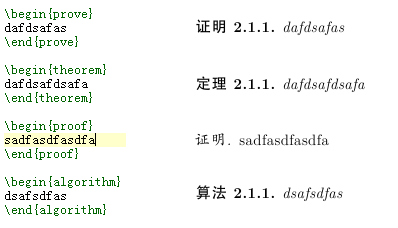
\includegraphics[scale=1]{figures/proofandprove}}
  \figcaption{proof、prove以及部分其他数学环境的差异}
  \label{pic:proofandprove}
\end{figure}


\section{模板提供的新命令}
主要的新命令如下:
\begin{description}
\item[\textbackslash figcaption\{\}]{效果是无论是否在图形环境中均生成图标题}
\item[\textbackslash tabcaption\{\}]{效果是无论是否在表格环境中均生成表标题}
\item[\textbackslash scite\{\}]{效果是得到如\scite{deng:01}这样的参考文献上标引用}
\item[\textbackslash chuhao]{改变字体大小为初号,类似的有\verb|\xiaoyihao|(小一号)直到\verb|\qihao|(七号)}
\item[\textbackslash makecover]{制作封面,供制本厂制作封面使用}
\item[\textbackslash maketitle]{制作扉页,中英文标题在一起}
\item[\textbackslash makeseparatetitle]{制作独立的中英文封面,中英文封面各一张\footnote{对于扉页格式,教务处没有规定,根据喜好二选一即可,或者自行发挥}}
\item[\textbackslash titletail\{\}]{中文标题过长的部分放在这个命令之中}
\item[\textbackslash tutor\{\}]{导师信息}
\item[\textbackslash entitle\{\}]{英文标题}
\item[\textbackslash entutor\{\}]{导师英文信息}
\item[\textbackslash cntime\{\}]{论文完成中文时间,自己填写}
\item[\textbackslash entime\{\}]{论文完成英文时间,自己填写}
\item[\textbackslash department\{\}]{院系中文名称}
\item[\textbackslash No\{\}]{学号}
\item[\textbackslash keywords\{\}]{英文关键字,在英文摘要环境中使用}
\item[\textbackslash cnkeywords\{\}]{中文关键字,在中文摘要环境中使用}
\item[\textbackslash L\{width\}]{表格环境中使用。对表格环境下p{width}命令进行加强,类似的还有C\{width\}和R\{width\}可以在指定宽度的同时指定对齐方式,三个命令分别表示左对齐、居中对齐、右对齐。注意大小写。(范例如下,效果如\autoref{tab:newcmd})}
\end{description}

\begin{minipage}{\textwidth}
\begin{verbatim}
\begin{table}
\tabcaption{几种命令效果对比的对比}
\label{tab:newcmd}
\centering
\begin{tabular}{c||l|c|r|p{2.5cm}|L{2.5cm}|C{2.5cm}|R{2.5cm}}
\hline
命令&l&c&r&p\{width\}&L\{width\}&C\{width\}&R\{width\}\\
\hline
效果&左齐&居中&右齐&定宽&左齐定宽&居中定宽&右齐定宽\\
\hline
\end{tabular}
\end{table}
\end{verbatim}

\tabcaption{几种命令效果对比的对比}
\label{tab:newcmd}
\centering
\begin{tabular}{c||l|c|r|p{2.5cm}|L{2.5cm}|C{2.5cm}|R{2.5cm}}
\hline
命令&l&c&r&p\{width\}&L\{width\}&C\{width\}&R\{width\}\\
\hline
效果&左齐&居中&右齐&定宽&左齐定宽&居中定宽&右齐定宽\\
\hline
\end{tabular}
\end{minipage}


\section{使用模板的一些注意事项}
把题目写在\verb|\title{}|中,只有题目过长的时候,再将过长的部分放在\verb|\titletail{}|中去(如\autoref{pic:title})。 

\begin{figure}
\centering
  \framebox{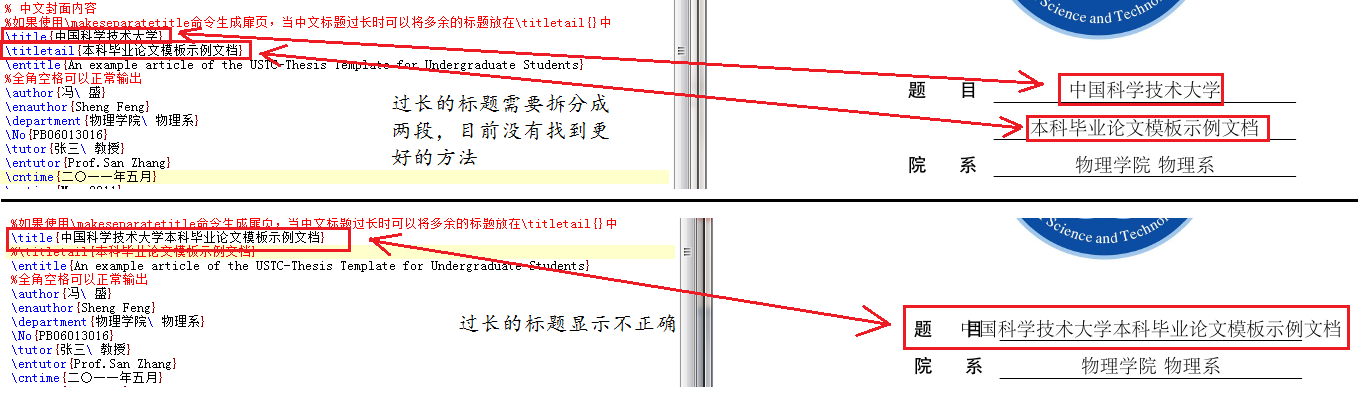
\includegraphics[scale=0.4]{figures/title}}
  \figcaption{过长的标题}
  \label{pic:title}
\end{figure}

比如:

对于短的题目——\\ \rule{4em}{0pt}\textbackslash title\{较短的题目\} 

对于较长的题目——\\\rule{4em}{0pt}\textbackslash title\{较长的题目的前一部分\} 
\\\rule{4em}{0pt}\textbackslash titletail\{较长的题目的后一部分\}

公式、章节、图和表格等(不包括脚注和参考文献)的交叉引用可以使用 \verb|\autoref{label}|来得到正确的引用。例如使用 \verb|\autoref{some_pic}|可以得到“图 X”的引用,使用 \verb|\autoref{some_table}|可以得到“表 X”的引用。

建议使用 \verb|\figcaption{}|命令得到所有图形的标题,表格也是。这样无论是否在图形环境中均能够得到正确的带图/表编号的标题,而在图形环境之外使用 \verb|\caption{}|命令会报错。

封面是按照制本厂的要求制作的,其中行宽和行高都是固定的,中文标题最多占两行,英文标题最多占三行。如果您的题目超过了这个限制,请缩减题目长度,不要擅自修改模板中的相关配置参数。



\chapter{引言:\CTeX 系统的安装和使用}
\label{chap:introduction}

本模板(ustcthesis.cls)是按照教务处的本科论文要求做出的\LaTeX 模板,作者为XPS。\par
本文是使用上述模板生成的示例文档,目的在于帮助使用者熟悉该模板的使用方法,并且方便使用者学位论文的撰写。

\section{系统要求,\CTeX 安装}
本文只针对Windows环境下\CTeX 套装。至于Linux使用者,我觉得你们有能力解决自己的问题。\par
如果电脑上尚未安装\LaTeX 系统,那么到\href{http://www.ctex.org/}{CTeX.org}下载最新完整版\CTeX 套装,并安装之。\par
此模板只支持UTF-8编码。将其他编码的文件转化为UTF-8的方法是: 用记事本打开这些文件, 然后点击文件—另存为—在最下方选择UTF-8 编码。在WinEdt中首次保存时,选择save as...,弹出的窗口中保存类型选择:UTF-8即可。


\section{WinEdit界面介绍和使用}
\CTeX 套装试用WinEdt作为默认编辑器,什么都配置好了,很方便,推荐使用。

打开\CTeX 套装内的WinEdit编辑器,可以看到如图\ref{f:winedit}的界面。
\begin{figure}[ht]
\centering
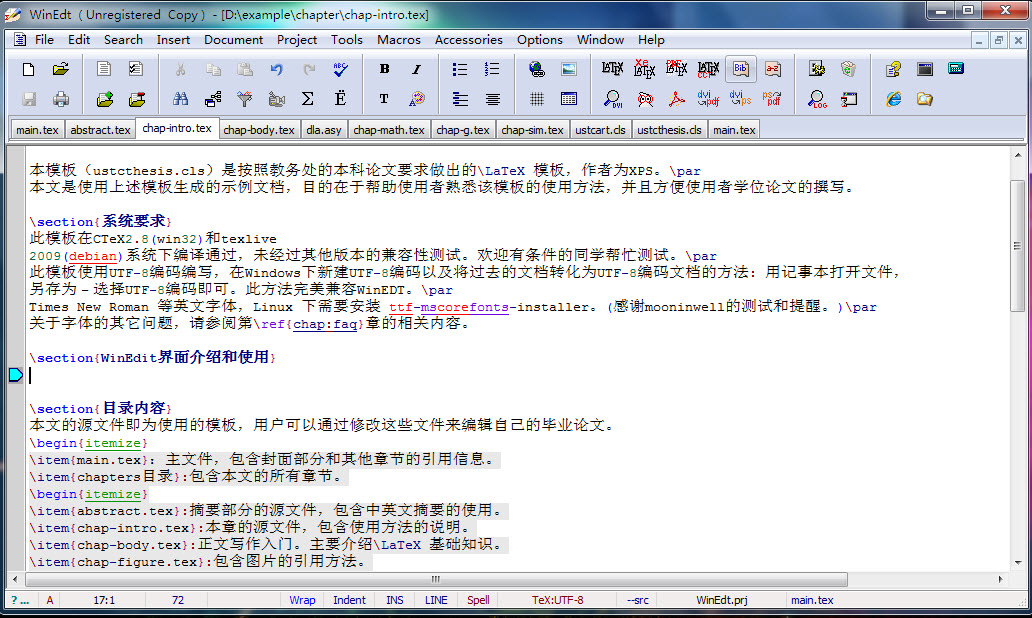
\includegraphics[width=0.8\textwidth]{winedit.jpg}
\caption{WinEdt界面}
\label{f:winedit}
\end{figure}

其中,中部的大块白色背景的区域就是键入文章内容的编辑区。编辑区上方的一条工具栏上有所有当前打开的文件的标签,单击即可跳转到对应文件。标签栏上方是面板,上面有一些很常用的工具按钮,鼠标悬停可以看到按钮名称。下面我们来看其中的几个。在使用本模板时,将会用到这些按钮。
\begin{itemize}
\item 
\includegraphics{open.jpg}\\
新建和打开按钮。
\item 
\includegraphics{mainfile.jpg}\\
单击左侧的按钮可设置主文件,单击右侧的取消主文件。
\item 
\includegraphics{mathhelp.jpg}\\
单击可以分别打开TeX SYMBOLS GUI(用于输入数学公式)和ASCII字符表。
\item 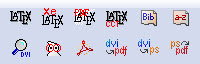
\includegraphics{compile.jpg}\\
编译区,我们需要使用的是上排第二个,第五个和下排第三个,即\XeLaTeX ,BibTeX和 Reader。
\end{itemize}

一般的写作流程是:准备好要写的文字和要插入的图片------在编辑区内输入文字------用各种\LaTeX 命令控制文章格式(第\ref{c:main}章),插入数学公式(第\ref{chap:math}章)、表格(第\ref{chap:tab}章)、图片(第\ref{chap:fig}章)等------编译(\ref{s:compile})------查看结果------修改,再编译------满意的文章。


\section{编译和调试方法}
\label{s:compile}
本模板需要使用\XeLaTeX 编译,切换到main.tex,点击面板上对应的按钮即可。如果你觉得每次都切过来很浪费时间,那么可以换到main.tex,并单击WinEdit工具栏上Set Main File按钮。这样的话以后每次编译都自动从main.tex开始,可以省掉不少麻烦。

如果编译出错,即停在某一位置不动了,且有问号提示符让使用者输入的话,那么按e回车,可以自动跳转到出错位置进行查看。出错的种类五花八门无法一一列举,但是一般都有详细的提示,如果有实在没法修正的可以到BBS TeX板提问。

编译通过之后,可以点工具栏上的Adobe按钮,打开预览。在CTeX2.8套装的WinEdit中,会弹出SumatraPDF,在这个窗口中,看到不合意的地方可以双击回到源文件的相应位置,逆向搜索到原文中的对应位置进行修改,还是比较方便的。\par

\begin{example}{Hello World}\\
将以下内容复制到新文件中,保存为\TeX 文件,编译,然后按Adobe按钮预览结果。
\begin{code}
    \documentclass{article}
    \begin{document}
        Hello world!
    \end{document}
\end{code}
\end{example}


为了得到正确的目录、交叉引用、参考文献等信息,需要编译两到三遍,正确的流程如下:
\begin{enumerate}
\item \XeLaTeX 编译一次。
\item BibTex编译一次。
\item \XeLaTeX 编译两到三次。
\end{enumerate}
在本示例文档中,提供了make.bat,双击之即可完成以上工作。



\section{目录内容}
本文的源文件即为使用的模板,用户可以通过修改这些文件来编辑自己的毕业论文。
\begin{itemize}
\item{main.tex}:主文件,包含封面部分和其他章节的引用信息。
\item{chapters目录}:包含本文的所有章节。
\begin{itemize}
\item{abstract.tex}:摘要部分的源文件,包含中英文摘要的使用。
\item{chap-intro.tex}:本章的源文件,包含使用方法的说明。
\item{chap-body.tex}:正文写作入门。主要介绍\LaTeX 基础知识。
\item{chap-figure.tex}:包含图片的引用方法。
\item{chap-table.tex}:包含表格的示例。
\item{chap-math.tex}:包含数学公式排版的基础知识。
\item{chap-app.tex}:附录。
\item{thanks.tex}包含致谢部分。
\end{itemize}
\item{figures目录}:存放文章内所用的图像文件。
\item{bib/tex.bib}:参考文献信息。
\end{itemize}
需要特别说明的是,这些文件名并不是固定的,你可以新建一个tex文件,例如zhangsan.tex,放在chapters目录下,并且在main.tex中使用
\begin{code}
    \include{chapters/zhangsan.tex}
\end{code}
来引用之。当然你也可以重命名这些文件,只要include中的文件名是存在的,\LaTeX 总能找到这些文件的。

在你写作某一章节的时候,你可能需要随时预览排版效果并debug,这时你可以在其他章节的\verb|\include|命令前加上一个\%,这代表注释掉本行,例如:
\begin{code}
    %%%%%%%%%%%%%%%%%%%%%%%%%%%%%%
    %% 正文部分
    %%%%%%%%%%%%%%%%%%%%%%%%%%%%%%
    \mainmatter
      
\chapter{引言:\CTeX 系统的安装和使用}
\label{chap:introduction}

本模板(ustcthesis.cls)是按照教务处的本科论文要求做出的\LaTeX 模板,作者为XPS。\par
本文是使用上述模板生成的示例文档,目的在于帮助使用者熟悉该模板的使用方法,并且方便使用者学位论文的撰写。

\section{系统要求,\CTeX 安装}
本文只针对Windows环境下\CTeX 套装。至于Linux使用者,我觉得你们有能力解决自己的问题。\par
如果电脑上尚未安装\LaTeX 系统,那么到\href{http://www.ctex.org/}{CTeX.org}下载最新完整版\CTeX 套装,并安装之。\par
此模板只支持UTF-8编码。将其他编码的文件转化为UTF-8的方法是: 用记事本打开这些文件, 然后点击文件—另存为—在最下方选择UTF-8 编码。在WinEdt中首次保存时,选择save as...,弹出的窗口中保存类型选择:UTF-8即可。


\section{WinEdit界面介绍和使用}
\CTeX 套装试用WinEdt作为默认编辑器,什么都配置好了,很方便,推荐使用。

打开\CTeX 套装内的WinEdit编辑器,可以看到如图\ref{f:winedit}的界面。
\begin{figure}[ht]
\centering
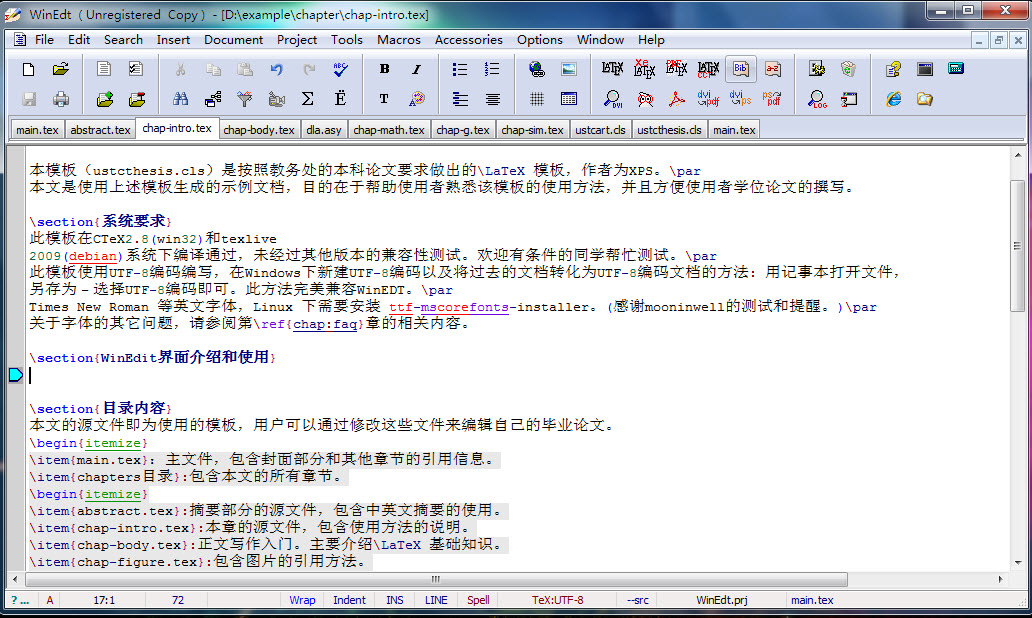
\includegraphics[width=0.8\textwidth]{winedit.jpg}
\caption{WinEdt界面}
\label{f:winedit}
\end{figure}

其中,中部的大块白色背景的区域就是键入文章内容的编辑区。编辑区上方的一条工具栏上有所有当前打开的文件的标签,单击即可跳转到对应文件。标签栏上方是面板,上面有一些很常用的工具按钮,鼠标悬停可以看到按钮名称。下面我们来看其中的几个。在使用本模板时,将会用到这些按钮。
\begin{itemize}
\item 
\includegraphics{open.jpg}\\
新建和打开按钮。
\item 
\includegraphics{mainfile.jpg}\\
单击左侧的按钮可设置主文件,单击右侧的取消主文件。
\item 
\includegraphics{mathhelp.jpg}\\
单击可以分别打开TeX SYMBOLS GUI(用于输入数学公式)和ASCII字符表。
\item 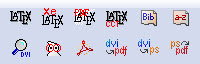
\includegraphics{compile.jpg}\\
编译区,我们需要使用的是上排第二个,第五个和下排第三个,即\XeLaTeX ,BibTeX和 Reader。
\end{itemize}

一般的写作流程是:准备好要写的文字和要插入的图片------在编辑区内输入文字------用各种\LaTeX 命令控制文章格式(第\ref{c:main}章),插入数学公式(第\ref{chap:math}章)、表格(第\ref{chap:tab}章)、图片(第\ref{chap:fig}章)等------编译(\ref{s:compile})------查看结果------修改,再编译------满意的文章。


\section{编译和调试方法}
\label{s:compile}
本模板需要使用\XeLaTeX 编译,切换到main.tex,点击面板上对应的按钮即可。如果你觉得每次都切过来很浪费时间,那么可以换到main.tex,并单击WinEdit工具栏上Set Main File按钮。这样的话以后每次编译都自动从main.tex开始,可以省掉不少麻烦。

如果编译出错,即停在某一位置不动了,且有问号提示符让使用者输入的话,那么按e回车,可以自动跳转到出错位置进行查看。出错的种类五花八门无法一一列举,但是一般都有详细的提示,如果有实在没法修正的可以到BBS TeX板提问。

编译通过之后,可以点工具栏上的Adobe按钮,打开预览。在CTeX2.8套装的WinEdit中,会弹出SumatraPDF,在这个窗口中,看到不合意的地方可以双击回到源文件的相应位置,逆向搜索到原文中的对应位置进行修改,还是比较方便的。\par

\begin{example}{Hello World}\\
将以下内容复制到新文件中,保存为\TeX 文件,编译,然后按Adobe按钮预览结果。
\begin{code}
    \documentclass{article}
    \begin{document}
        Hello world!
    \end{document}
\end{code}
\end{example}


为了得到正确的目录、交叉引用、参考文献等信息,需要编译两到三遍,正确的流程如下:
\begin{enumerate}
\item \XeLaTeX 编译一次。
\item BibTex编译一次。
\item \XeLaTeX 编译两到三次。
\end{enumerate}
在本示例文档中,提供了make.bat,双击之即可完成以上工作。



\section{目录内容}
本文的源文件即为使用的模板,用户可以通过修改这些文件来编辑自己的毕业论文。
\begin{itemize}
\item{main.tex}:主文件,包含封面部分和其他章节的引用信息。
\item{chapters目录}:包含本文的所有章节。
\begin{itemize}
\item{abstract.tex}:摘要部分的源文件,包含中英文摘要的使用。
\item{chap-intro.tex}:本章的源文件,包含使用方法的说明。
\item{chap-body.tex}:正文写作入门。主要介绍\LaTeX 基础知识。
\item{chap-figure.tex}:包含图片的引用方法。
\item{chap-table.tex}:包含表格的示例。
\item{chap-math.tex}:包含数学公式排版的基础知识。
\item{chap-app.tex}:附录。
\item{thanks.tex}包含致谢部分。
\end{itemize}
\item{figures目录}:存放文章内所用的图像文件。
\item{bib/tex.bib}:参考文献信息。
\end{itemize}
需要特别说明的是,这些文件名并不是固定的,你可以新建一个tex文件,例如zhangsan.tex,放在chapters目录下,并且在main.tex中使用
\begin{code}
    \include{chapters/zhangsan.tex}
\end{code}
来引用之。当然你也可以重命名这些文件,只要include中的文件名是存在的,\LaTeX 总能找到这些文件的。

在你写作某一章节的时候,你可能需要随时预览排版效果并debug,这时你可以在其他章节的\verb|\include|命令前加上一个\%,这代表注释掉本行,例如:
\begin{code}
    %%%%%%%%%%%%%%%%%%%%%%%%%%%%%%
    %% 正文部分
    %%%%%%%%%%%%%%%%%%%%%%%%%%%%%%
    \mainmatter
      
\chapter{引言:\CTeX 系统的安装和使用}
\label{chap:introduction}

本模板(ustcthesis.cls)是按照教务处的本科论文要求做出的\LaTeX 模板,作者为XPS。\par
本文是使用上述模板生成的示例文档,目的在于帮助使用者熟悉该模板的使用方法,并且方便使用者学位论文的撰写。

\section{系统要求,\CTeX 安装}
本文只针对Windows环境下\CTeX 套装。至于Linux使用者,我觉得你们有能力解决自己的问题。\par
如果电脑上尚未安装\LaTeX 系统,那么到\href{http://www.ctex.org/}{CTeX.org}下载最新完整版\CTeX 套装,并安装之。\par
此模板只支持UTF-8编码。将其他编码的文件转化为UTF-8的方法是: 用记事本打开这些文件, 然后点击文件—另存为—在最下方选择UTF-8 编码。在WinEdt中首次保存时,选择save as...,弹出的窗口中保存类型选择:UTF-8即可。


\section{WinEdit界面介绍和使用}
\CTeX 套装试用WinEdt作为默认编辑器,什么都配置好了,很方便,推荐使用。

打开\CTeX 套装内的WinEdit编辑器,可以看到如图\ref{f:winedit}的界面。
\begin{figure}[ht]
\centering
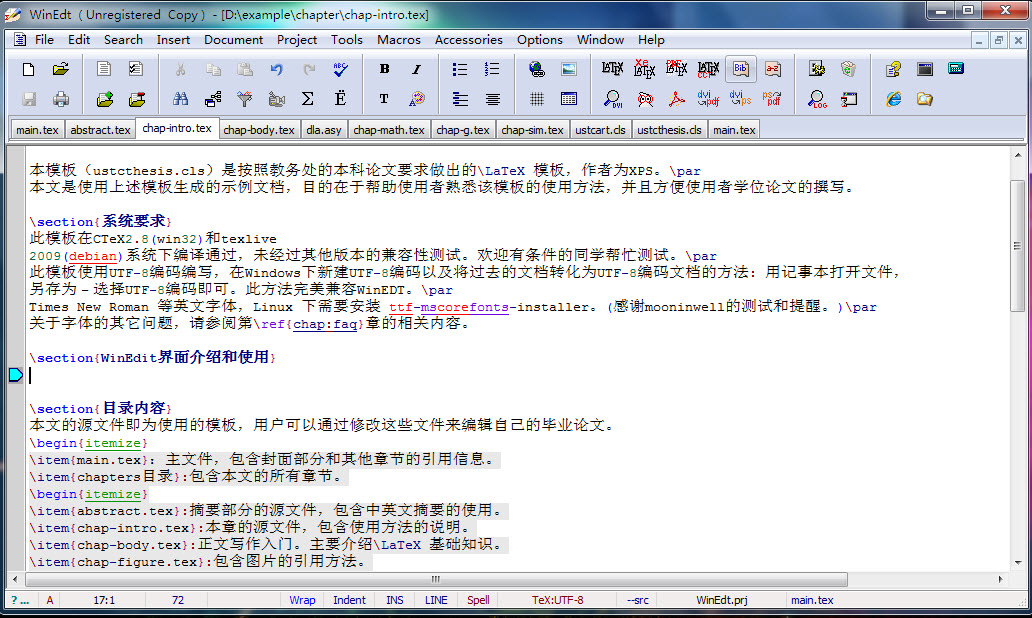
\includegraphics[width=0.8\textwidth]{winedit.jpg}
\caption{WinEdt界面}
\label{f:winedit}
\end{figure}

其中,中部的大块白色背景的区域就是键入文章内容的编辑区。编辑区上方的一条工具栏上有所有当前打开的文件的标签,单击即可跳转到对应文件。标签栏上方是面板,上面有一些很常用的工具按钮,鼠标悬停可以看到按钮名称。下面我们来看其中的几个。在使用本模板时,将会用到这些按钮。
\begin{itemize}
\item 
\includegraphics{open.jpg}\\
新建和打开按钮。
\item 
\includegraphics{mainfile.jpg}\\
单击左侧的按钮可设置主文件,单击右侧的取消主文件。
\item 
\includegraphics{mathhelp.jpg}\\
单击可以分别打开TeX SYMBOLS GUI(用于输入数学公式)和ASCII字符表。
\item 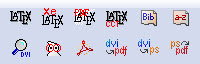
\includegraphics{compile.jpg}\\
编译区,我们需要使用的是上排第二个,第五个和下排第三个,即\XeLaTeX ,BibTeX和 Reader。
\end{itemize}

一般的写作流程是:准备好要写的文字和要插入的图片------在编辑区内输入文字------用各种\LaTeX 命令控制文章格式(第\ref{c:main}章),插入数学公式(第\ref{chap:math}章)、表格(第\ref{chap:tab}章)、图片(第\ref{chap:fig}章)等------编译(\ref{s:compile})------查看结果------修改,再编译------满意的文章。


\section{编译和调试方法}
\label{s:compile}
本模板需要使用\XeLaTeX 编译,切换到main.tex,点击面板上对应的按钮即可。如果你觉得每次都切过来很浪费时间,那么可以换到main.tex,并单击WinEdit工具栏上Set Main File按钮。这样的话以后每次编译都自动从main.tex开始,可以省掉不少麻烦。

如果编译出错,即停在某一位置不动了,且有问号提示符让使用者输入的话,那么按e回车,可以自动跳转到出错位置进行查看。出错的种类五花八门无法一一列举,但是一般都有详细的提示,如果有实在没法修正的可以到BBS TeX板提问。

编译通过之后,可以点工具栏上的Adobe按钮,打开预览。在CTeX2.8套装的WinEdit中,会弹出SumatraPDF,在这个窗口中,看到不合意的地方可以双击回到源文件的相应位置,逆向搜索到原文中的对应位置进行修改,还是比较方便的。\par

\begin{example}{Hello World}\\
将以下内容复制到新文件中,保存为\TeX 文件,编译,然后按Adobe按钮预览结果。
\begin{code}
    \documentclass{article}
    \begin{document}
        Hello world!
    \end{document}
\end{code}
\end{example}


为了得到正确的目录、交叉引用、参考文献等信息,需要编译两到三遍,正确的流程如下:
\begin{enumerate}
\item \XeLaTeX 编译一次。
\item BibTex编译一次。
\item \XeLaTeX 编译两到三次。
\end{enumerate}
在本示例文档中,提供了make.bat,双击之即可完成以上工作。



\section{目录内容}
本文的源文件即为使用的模板,用户可以通过修改这些文件来编辑自己的毕业论文。
\begin{itemize}
\item{main.tex}:主文件,包含封面部分和其他章节的引用信息。
\item{chapters目录}:包含本文的所有章节。
\begin{itemize}
\item{abstract.tex}:摘要部分的源文件,包含中英文摘要的使用。
\item{chap-intro.tex}:本章的源文件,包含使用方法的说明。
\item{chap-body.tex}:正文写作入门。主要介绍\LaTeX 基础知识。
\item{chap-figure.tex}:包含图片的引用方法。
\item{chap-table.tex}:包含表格的示例。
\item{chap-math.tex}:包含数学公式排版的基础知识。
\item{chap-app.tex}:附录。
\item{thanks.tex}包含致谢部分。
\end{itemize}
\item{figures目录}:存放文章内所用的图像文件。
\item{bib/tex.bib}:参考文献信息。
\end{itemize}
需要特别说明的是,这些文件名并不是固定的,你可以新建一个tex文件,例如zhangsan.tex,放在chapters目录下,并且在main.tex中使用
\begin{code}
    \include{chapters/zhangsan.tex}
\end{code}
来引用之。当然你也可以重命名这些文件,只要include中的文件名是存在的,\LaTeX 总能找到这些文件的。

在你写作某一章节的时候,你可能需要随时预览排版效果并debug,这时你可以在其他章节的\verb|\include|命令前加上一个\%,这代表注释掉本行,例如:
\begin{code}
    %%%%%%%%%%%%%%%%%%%%%%%%%%%%%%
    %% 正文部分
    %%%%%%%%%%%%%%%%%%%%%%%%%%%%%%
    \mainmatter
      \include{chapter/chap-intro}
    %  \include{chapter/chap-figure}
    %  \include{chapter/chap-table}
    %  \include{chapter/chap-math}
    %  \include{chapter/chap-faq}
\end{code}
那么,编译的时候就只编译未加\%的一章,在这个例子中,即本章。

理论上,并不一定要把每章放在不同的文件中,但是这种分章节写作、编译的方法有利于提高效率,大大减少debug过程中的编译时间,同时减小风险。 
    %  
\chapter{图形}
\label{chap:fig}


\section{浮动图形}

\XeLaTeX 支持jpg和eps格式的图片。我们所用的编译方法支持jpg和eps等格式的图片。如果你已经有一篇word文档,
想把其中的图全部导出,那么可以将它另存为html文件,这时会在同目录下找到一个文件夹,里面是所有用到的图片。

将插图放在figures文件夹中,想要引用的地方使用类似这样的命令插入图形文件:
\begin{code}
\begin{figure}[!ht]
 \centering
 
\includegraphics[width=0.2\textwidth]{ustc_logo_new.eps}
 \caption{中国科学技术大学校徽(在页面中间)}
 \label{fig:ustc1}
\end{figure}
\end{code}
结果如下:
\begin{figure}[!ht]
 \centering
 
\includegraphics[width=0.2\textwidth]{ustc_logo_new.eps}
 \caption{中国科学技术大学校徽(在页面中间)}
 \label{fig:ustc1}
\end{figure}

在上面这段命令中,可选参数[!ht]代表插图的位置。其中!让\LaTeX{}忽略审美标准,试图用最严格的标准来放置浮动图形;h(ere)代表有限放在此处;t(op)代表如果此处放不下,那么放在下一页页首。

width=0.2\textbackslash{}textwidth代表图形的宽度是文字宽度的0.2倍,你也可以使用其他长度单位,如12cm,4.5in等等。

caption命令的参数代表图的名称,或者说注解。label的参数用于交叉引用,见下节。


\section{交叉引用}
通过使用交叉引用功能,我们可以定位那些\LaTeX{}自动编号的内容,比如浮动图形、表格、章节等等。其中,label和ref的参数是引用的名字,可以随意,但须保持一致。
\begin{figure}[ht]
\centering
\fbox{\begin{minipage}[h]{0.4\textwidth}
引用图\ref{fig:ustc1}\\
引用第\ref{chap:introduction}章
\end{minipage}}
\hspace{0.1\textwidth}
\begin{minipage}[h]{0.4\textwidth}
\centering
\begin{code}
引用图\ref{fig:ustc1}\\
引用第\ref{chap:introduction}章
\end{code}
\end{minipage}
\caption{交叉引用示例}
\end{figure}


\section{并列的子图}
使用subfigure命令,一个例子:
\begin{figure}[!hbt]
\centering
\subfigure[sf 1]{

\includegraphics[width=0.2\textwidth]{ustc_logo_new.eps}\label{f:1}}
\subfigure[sf 2]{

\includegraphics[width=0.2\textwidth]{ustc_logo_new.eps}\label{f:2}}
\subfigure[sf 3]{

\includegraphics[width=0.2\textwidth]{ustc_logo_new.eps}\label{f:3}}
\subfigure[sf 4]{

\includegraphics[width=0.2\textwidth]{ustc_logo_new.eps}\label{f:4}}
\caption{\label{f:s}subfigure使用示例。}
\end{figure}
\begin{code}
\begin{figure}[!hbt]
\centering
\subfigure[sf 1]{

\includegraphics[width=0.2\textwidth]{ustc_logo_new.eps}\label{f:1}}
\subfigure[sf 2]{

\includegraphics[width=0.2\textwidth]{ustc_logo_new.eps}\label{f:2}}
\subfigure[sf 3]{

\includegraphics[width=0.2\textwidth]{ustc_logo_new.eps}\label{f:3}}
\subfigure[sf 4]{

\includegraphics[width=0.2\textwidth]{ustc_logo_new.eps}\label{f:4}}
\caption{\label{f:s}subfigure使用示例。}
\end{figure}
\end{code}

分两行放:
\begin{figure}[!hbt]
\centering
\subfigure[sf 1]{

\includegraphics[width=0.2\textwidth]{ustc_logo_new.eps}\label{f:1}}
\subfigure[sf 2]{

\includegraphics[width=0.2\textwidth]{ustc_logo_new.eps}\label{f:2}}\\
\subfigure[sf 3]{

\includegraphics[width=0.2\textwidth]{ustc_logo_new.eps}\label{f:3}}
\subfigure[sf 4]{

\includegraphics[width=0.2\textwidth]{ustc_logo_new.eps}\label{f:4}}
\caption{\label{f:s}subfigure使用示例。}
\end{figure}
\begin{code}
\begin{figure}[!hbt]
\centering
\subfigure[f 1]{

\includegraphics[width=0.2\textwidth]{ustc_logo_new.eps}\label{f:1}}
\subfigure[f 2]{

\includegraphics[width=0.2\textwidth]{ustc_logo_new.eps}\label{f:2}}\\
\subfigure[f 3]{

\includegraphics[width=0.2\textwidth]{ustc_logo_new.eps}\label{f:3}}
\subfigure[f 4]{

\includegraphics[width=0.2\textwidth]{ustc_logo_new.eps}\label{f:4}}
\caption{\label{f:l}分行的字图使用示例。}
\end{figure}
\end{code}
    %  
\chapter{表格}
\label{chap:tab}
标准三线表:
\begin{table}[!ht]
\label{tab:table3}
\caption{三线表格示例}
\centering
\begin{tabular}{c c c c}
\whline 一列 & 两列 & 三列 & 四列  \\\hline
1 & 2 &3 &4 \\2 & 3 &4 &5 \\3 & 4 &5 &6 \\
\whline
\end{tabular}
\end{table}
\begin{code}
    \begin{table}[!ht]
    \label{tab:table3}
    \caption{三线表格示例}
    \centering
    \begin{tabular}{c c c c}
        \whline 一列 & 两列 & 三列 & 四列  \\\whline
        1 & 2 &3 &4 \\2 & 3 &4 &5 \\3 & 4 &5 &6 \\
        \whline
    \end{tabular}
    \end{table}
\end{code}

与figure一样,table环境也是浮动体,常用!ht来表明位置。caption、label的意义都与figure环境相同。

而画表格的tabular环境则与array环境几乎相同,只是在每行之间可以用\textbackslash{}hline和\textbackslash{}hline这些命令来画横线。c代表一个居中对齐的列,l代表靠左对齐,r代表靠右对齐。
有竖线的例子:
\begin{table}[!ht]
\label{tab:table2}
\caption{表格示例2}
\centering
\begin{tabular}{ Ic|c|c|cI}
\whline 一列 & 两列 & 三列 & 四列  \\\hline
1 & 2 &3 &4 \\\hline 2 & 3 &4 &5 \\\hline3 & 4 &5 &6 \\
\whline
\end{tabular}
\end{table}
\begin{code}
    \begin{table}[!ht]
    \label{tab:table2}
    \caption{表格示例2}
    \centering
    \begin{tabular}{ Ic|c|c|cI}
        \whline 一列 & 两列 & 三列 & 四列  \\\hline
        1 & 2 &3 &4 \\\hline 2 & 3 &4 &5 \\\hline3 & 4 &5 &6 \\
        \whline
    \end{tabular}
    \end{table}
\end{code}

即竖线是|,粗竖线是大写字母I,横线是\textbackslash hline,粗横线是\textbackslash whline。

    %  
\chapter{数学公式}
\label{chap:math}
数学公式需在数学环境中排版。数学环境一般分\textit{正文公式}和\textit{显示公式}。正文公式用\verb|$...$|表示,而显示公式则用equation,align等数学环境。简单的几个例子:
\begin{figure}[ht]
\centering
\fbox{\begin{minipage}[h]{0.4\textwidth}
这是一个显示公式:
    \begin{equation}
    x+y=z
    \end{equation}
谢谢。
\end{minipage}}
\hspace{0.1\textwidth}
\begin{minipage}[h]{0.4\textwidth}
\centering
\begin{code}
这是一个显示公式:
\begin{equation}
x+y=z
\end{equation}
谢谢。
\end{code}
\end{minipage}
\caption{显示公式}
\end{figure}
\begin{figure}[h]
\centering
\fbox{\begin{minipage}[c]{0.4\textwidth}
大家好,$e^{\pi i}+1=0$是我最喜欢的方程。
\end{minipage}}
\hspace{0.1\textwidth}
\begin{minipage}[h]{0.4\textwidth}
\centering
\begin{code}
大家好,$e^{\pi i}+1=0$是我最喜欢的方程。
\end{code}
\end{minipage}
\caption{正文公式}
\end{figure}

常用的显示公式环境有:
\begin{itemize}
\item{equation}:最常用的公式环境。
\item{displaymath}:与equation的差别在于不会被自动编号。\\
\verb|\begin{displaymath}...\end{displaymath}|可以用\verb|\[...\]|来代替。
\item{align}:适用于排版多个需要对齐的公式。
\end{itemize}


\section{数学公式排版基础}
上下标、希腊字母、加减乘除等常用符号:
\begin{center}
\begin{tabular}{ccll}
\whline
& 命令 & 例子 & 代码\\
\hline
上标 & \^{} & $x^2$ & \verb|$x^2$|\\
下标 & \_{} & $x_2$ & \verb|$x_2$|\\
希腊字母 & 对应的英文 & $\pi,\rho,\sigma,...$ &\verb|$\pi,\rho,\sigma,...$|\\
点乘 & \verb|\cdot| & $x\cdot y$ & \verb|$x\cdot y$|\\
叉乘 & \verb|\times| & $x\times y$ & \verb|$x\times y$|\\
分数 & \verb|\frac{}{}| & $\frac{abc}{def}$ &\verb|$\frac{abc}{def}$|\\
根号 & \verb|\sqrt[n]{}|  & $\sqrt{x},\sqrt[3]{y}$ &\verb|$\sqrt{x},\sqrt[3]{y}$|\\
积分 &\verb|\int|  & $\int,\iint,\iiint$ & \verb|$\int,\iint,\iiint$|\\
\whline
\end{tabular}
\end{center}
表中,\$代表数学环境。在equation等环境中排版时,不再需要使用\$符号。

更多的符号,请点击WinEdt面板上的$\Sigma$符号(TeX Symbols GUI),在弹出的面板中查找。

当控制符作用于多个字符时,需要用大括号将这些字符都括起来,如
\begin{center}
\begin{tabular}{c c}
\whline
例子 & 代码\\
\hline
$e^{\pi i}+1=0$ & \verb|e^{\pi i}+1=0|\\
$x_{12}^{3}$ & \verb|x_{12}^{3}|\\
${x_{12}}^{3}$ & \verb|{x_{12}}^{3}|\\
\whline
\end{tabular}
\end{center}

\section{控制字体}
本科学位论文对于公式内字体的使用有严格的规定。一般变量用白斜体,常量和特殊函数等用白正体,矢量用黑斜体,张量用黑正体。改变字体的命令如下表:
\begin{center}
\begin{tabular}{c c l l}
\whline
& 字体 & 例子 & 代码\\
\hline
一般变量 & 白斜体 & $x$ & \verb|$x$|\\
常量  & 白正体 & $\mathrm{c}$  & \verb|$\mathrm{c}$|\\
矢量  & 黑斜体 & $\bm{B}$ & \verb|$\bm{B}$|\\
张量  & 黑正体 & $\mathbf{H}$ & \verb|$\mathbf{H}$|\\
\whline
\end{tabular}
\end{center}
表中,\$代表数学环境。在equation等环境中排版时,不再需要使用\$符号。

\section{括号}
中括号、小括号和竖线可以用键盘上对应的键来输入。大括号是\LaTeX{}中的控制符,必须用\verb|\{...\}|来输入。态函数所用的尖括号是\verb|\langle|和\verb|\rangle|。一个句点代表一个不显示的括号。

使用\verb|\left|和\verb|\right|可以自动控制括号的大小。使用时,将所需要用的括号紧跟在\verb|\left|或\verb|\right|后面就好。例如:
\begin{figure}[ht]
\centering
\fbox{\begin{minipage}[h]{0.8\textwidth}
    \[
    \left[\frac{\left(\frac{abc}{def}+ghi\right)\cdot jkl}{mno}+pqr\right]\times st=0
    \]
\end{minipage}}\\
\vskip10pt
\begin{minipage}[h]{0.8\textwidth}
\centering
\begin{code}
\[
\left[\frac{\left(\frac{abc}{def}+ghi\right)\cdot jkl}{mno}+pqr\right]
\times st=0
\]
\end{code}
\end{minipage}
\caption{括号。\textbackslash[和\textbackslash]代表displaymath环境,下同。}
\end{figure}



使用括号时,不一定要用相同的括号来匹配。甚至可以用\verb|\left.|这样不被显示括号来匹配正常括号,以达到排版目的。如
\begin{figure}[h]
\centering
\fbox{\begin{minipage}[h]{0.4\textwidth}
\[\left|\psi\right\rangle\]
\end{minipage}}
\hspace{0.1\textwidth}
\begin{minipage}[h]{0.4\textwidth}
\centering
\begin{code}
\[\left|\psi\right\rangle\]
\end{code}
\end{minipage}\\
\vskip10pt
\fbox{\begin{minipage}[h]{0.4\textwidth}
\[\left\{
\begin{array}{c}
a\\b\\c
\end{array}
\right.\]
\end{minipage}}
\hspace{0.1\textwidth}
\begin{minipage}[h]{0.4\textwidth}
\centering
\begin{code}
\[\left\{\begin{array}{c}
a\\b\\c
\end{array}\right.\]
\end{code}
\end{minipage}
\caption{不同括号的匹配}
\end{figure}

\section{矩阵}
输入矩阵一般使用array环境。

矩阵中使用\verb|&|来分位,\verb|\\|来分行。array环境的参数指定了列的数量和每列的对齐方式。c代表一个居中对齐的列,l是靠左对齐,r则是靠右对齐。图\ref{f:matrix}是一个简单的例子。
\begin{figure}[h]
\centering
\fbox{\begin{minipage}[h]{0.4\textwidth}
\[\left[
\begin{array}{c c c}
C_{Xx} & C_{Yx} & C_{Zx}\\
C_{Xy} & C_{Yy} & C_{Zy}\\
C_{Xz} & C_{Yz} & C_{Zz}
\end{array}
\right]\]
\end{minipage}}
\hspace{0.1\textwidth}
\begin{minipage}[h]{0.4\textwidth}
\centering
\begin{code}
\[\left[\begin{array}{c c c}
C_{Xx} & C_{Yx} & C_{Zx}\\
C_{Xy} & C_{Yy} & C_{Zy}\\
C_{Xz} & C_{Yz} & C_{Zz}
\end{array}\right]\]
\end{code}
\end{minipage}
\caption{矩阵}
\label{f:matrix}
\end{figure}

array环境可以自嵌套,达到输入复杂矩阵的目的。

\section{对齐的多行公式}
align环境提供了书写多行公式,并指定其在某一位置对齐的功能,使用\&来代表对齐点。如图\ref{f:align}。其中,\verb|\notag| 表示不对这一行公式进行编号。
\begin{figure}[h]
\centering
\fbox{\begin{minipage}[b]{0.8\textwidth}
\begin{align}
a_0&=(A_1+A_2+A_3)/3\textrm{g}_e\beta_e\\
b_0&=[A_1-(A_2+A_3)/2]/3\textrm{g}_e\beta_e\notag\\
c_0&=(|A_2|-|A_3|)/2\textrm{g}_e\beta_e
\end{align}
\end{minipage}}\\
\begin{minipage}[b]{0.8\textwidth}
\centering
\begin{code}
\begin{align}
a_0&=(A_1+A_2+A_3)/3\textrm{g}_e\beta_e\\
b_0&=[A_1-(A_2+A_3)/2]/3\textrm{g}_e\beta_e\notag\\
c_0&=(|A_2|-|A_3|)/2\textrm{g}_e\beta_e
\end{align}
\end{code}
\end{minipage}
\caption{多行公式}
\label{f:align}
\end{figure}

\section{定理,证明,和其他环境}
ustcthesis中提供了定理,证明等一些其他环境。环境和名称如下表:
\begin{center}
\begin{tabular}{l l @\qquad l l}
\whline
环境名 & 中文名 &环境名 & 中文名\\
\hline
theorem & 定理&
lemma&引理\\
example&例&
algorithm&算法\\
definition&定义&
axiom&公理\\
property&性质&
proposition&命题\\
corollary&推论&
remark&注解\\
condition&条件&
conclusion&结论\\
assumption&假设&
prove&证明\\
\whline
\end{tabular}
\end{center}

    %  \def\Q{\noindent Question:~~}
\def\A{\newline Answer:~~}
\chapter{FAQ}
\label{chap:contact}

这里是我们已经收到的一些常见问题以及一些一般的Debug技巧. 对于更多的信息或者关于本模板和文档的任何疑问,请移步\href{http://bbs.ustc.edu.cn/cgi/bbsdoc?board=TeX}{瀚海星云\TeX{}讨论区}。

\Q 从哪里下载\CTeX{}套装? 应该下载哪一个\CTeX{}套装?
\A 在\href{http://www.ctex.org}{\CTeX{}官方网站}可以下载, 进入网站后点击网页右边的``项目''栏目中``最新稳定版'', 即可进入下载链接. 对于有良好网络链接的同学, 我们强烈建议下载较大的那个完全版, 实在是网络速度不佳的同学可以下载精简版的, 但是编译的时候会经常实时下载某些宏包, 很麻烦, 因此不推荐.

\Q 我自己新建了一个文件并且写了一段文字, 为什么编译出来的中文是乱码呢? 但是用模板里面的文件编译正常.
\A 请仔细确认你新建的文件是不是UTF-8编码! 如果不是, 请按文章前述方法转换成UTF-8编码.

\Q 我编译总是报错, 按e定位总是定位到主文件?
\A 这种问题比较复杂, 可能是你的某个正文中的命令与模板冲突, 或者有时与宏包冲突也会出现这种情况. 这时我们只能手动定位错误, 具体方式如下: 首先确定问题在哪一章? 方法是一章一章的编译, 然后确定问题在哪一节, 方法是只编译问题章节, 然后一节一节的编译. 最后确定问题在哪一行. 一般对于新手而言, 容易在数学公式中出问题, 所以, 请优先检查数学公式. 这样通过逐级定位, 我们就可以精确的获知错误的位置, 然后仔细检查, 就可以得到错误的原因, 即使你无法理解错误, 也可以对症求医, 在\TeX{}版求问.

\Q 编译错误时, DOS窗口里报了一大堆英文, 如何看懂啊?
\A 前面的都是编译信息不用理睬, 后面的是错误信息要仔细看, 比如这一段
\begin{code}
  ! Undefined control sequence.
l.16 \adga
           agasgarga
?
\end{code}
这一段有4行, 最后一行是问你如何处理, 我们在这里输入我们的处理方案. 现在看前三行. 第一行由一个感叹号开头, 这里是错误原因, 说明我用了一个没有定义的命令.
第二行是\verb|l.16|开头, 说明第16行出问题了, 然后这里有一个断行, 这个断行表示错误的精确位置, 这里, 由于没有\verb|\adga|这个命令, 自然就会报错.
后面的第三行是辅助文字, 表示错误后面的一些代码, 这样可以方便我们精确定位, 这种显示方式在大段的数学公式出错时尤其方便. 至于第4行, 前述办法是: 一般按E, 回车, 方便的在代码中回溯到我们需要的行. 在这里我们再介绍一个命令: h---回车. h的意思是help, 这样, \TeX{}的编译器会使用尽可能你熟悉的语言告诉你具体为什么错了. 有的时候这是很有帮助的, 而有的时候你却完全不知道他在说什么. 这是很正常的, 因为电脑的长处在于执行命令, 而不是主动读懂你的想法.(Knuth in TeXbook)

\Q 一个诡异的错误:
\A 也许你已经学习了一些公式的编写, 那么, 请看下面一段代码:
\begin{code}
\begin{eqnarray}
  [X_1, X_2] &=& 0\\
  [X_3, X_4] &=& Q_{\pm}
\end{eqnarray}
\end{code}
你肯定觉得这是个很简单的括号问题, 但是实际上这是无法编译的! 解决方案是在第一行公式后面加上\verb|\relax|, 原因很巧妙, 换行符\verb|\\|后面的中括号代表该命令的可选参数, 表示空多少尺寸, 在上述公式中, 第二行的公式恰好是以\verb|[|开头, 自然无法编译过去. 这在TeXbook中叫做``weird mistakes''. 其实, 我们有很多可能遇到各种诡异的问题, 有时这种问题的思路是超越我们的想法的, 因此, 希望大家可以多多发问, 善于在网络上与同学们讨论问题, 这样才能有助于问题的解决.



\end{code}
那么,编译的时候就只编译未加\%的一章,在这个例子中,即本章。

理论上,并不一定要把每章放在不同的文件中,但是这种分章节写作、编译的方法有利于提高效率,大大减少debug过程中的编译时间,同时减小风险。 
    %  
\chapter{图形}
\label{chap:fig}


\section{浮动图形}

\XeLaTeX 支持jpg和eps格式的图片。我们所用的编译方法支持jpg和eps等格式的图片。如果你已经有一篇word文档,
想把其中的图全部导出,那么可以将它另存为html文件,这时会在同目录下找到一个文件夹,里面是所有用到的图片。

将插图放在figures文件夹中,想要引用的地方使用类似这样的命令插入图形文件:
\begin{code}
\begin{figure}[!ht]
 \centering
 
\includegraphics[width=0.2\textwidth]{ustc_logo_new.eps}
 \caption{中国科学技术大学校徽(在页面中间)}
 \label{fig:ustc1}
\end{figure}
\end{code}
结果如下:
\begin{figure}[!ht]
 \centering
 
\includegraphics[width=0.2\textwidth]{ustc_logo_new.eps}
 \caption{中国科学技术大学校徽(在页面中间)}
 \label{fig:ustc1}
\end{figure}

在上面这段命令中,可选参数[!ht]代表插图的位置。其中!让\LaTeX{}忽略审美标准,试图用最严格的标准来放置浮动图形;h(ere)代表有限放在此处;t(op)代表如果此处放不下,那么放在下一页页首。

width=0.2\textbackslash{}textwidth代表图形的宽度是文字宽度的0.2倍,你也可以使用其他长度单位,如12cm,4.5in等等。

caption命令的参数代表图的名称,或者说注解。label的参数用于交叉引用,见下节。


\section{交叉引用}
通过使用交叉引用功能,我们可以定位那些\LaTeX{}自动编号的内容,比如浮动图形、表格、章节等等。其中,label和ref的参数是引用的名字,可以随意,但须保持一致。
\begin{figure}[ht]
\centering
\fbox{\begin{minipage}[h]{0.4\textwidth}
引用图\ref{fig:ustc1}\\
引用第\ref{chap:introduction}章
\end{minipage}}
\hspace{0.1\textwidth}
\begin{minipage}[h]{0.4\textwidth}
\centering
\begin{code}
引用图\ref{fig:ustc1}\\
引用第\ref{chap:introduction}章
\end{code}
\end{minipage}
\caption{交叉引用示例}
\end{figure}


\section{并列的子图}
使用subfigure命令,一个例子:
\begin{figure}[!hbt]
\centering
\subfigure[sf 1]{

\includegraphics[width=0.2\textwidth]{ustc_logo_new.eps}\label{f:1}}
\subfigure[sf 2]{

\includegraphics[width=0.2\textwidth]{ustc_logo_new.eps}\label{f:2}}
\subfigure[sf 3]{

\includegraphics[width=0.2\textwidth]{ustc_logo_new.eps}\label{f:3}}
\subfigure[sf 4]{

\includegraphics[width=0.2\textwidth]{ustc_logo_new.eps}\label{f:4}}
\caption{\label{f:s}subfigure使用示例。}
\end{figure}
\begin{code}
\begin{figure}[!hbt]
\centering
\subfigure[sf 1]{

\includegraphics[width=0.2\textwidth]{ustc_logo_new.eps}\label{f:1}}
\subfigure[sf 2]{

\includegraphics[width=0.2\textwidth]{ustc_logo_new.eps}\label{f:2}}
\subfigure[sf 3]{

\includegraphics[width=0.2\textwidth]{ustc_logo_new.eps}\label{f:3}}
\subfigure[sf 4]{

\includegraphics[width=0.2\textwidth]{ustc_logo_new.eps}\label{f:4}}
\caption{\label{f:s}subfigure使用示例。}
\end{figure}
\end{code}

分两行放:
\begin{figure}[!hbt]
\centering
\subfigure[sf 1]{

\includegraphics[width=0.2\textwidth]{ustc_logo_new.eps}\label{f:1}}
\subfigure[sf 2]{
\includegraphics[width=0.2\textwidth]{ustc_logo_new.eps}\label{f:2}}\\
\subfigure[sf 3]{
\includegraphics[width=0.2\textwidth]{ustc_logo_new.eps}\label{f:3}}
\subfigure[sf 4]{
\includegraphics[width=0.2\textwidth]{ustc_logo_new.eps}\label{f:4}}
\caption{\label{f:s}subfigure使用示例。}
\end{figure}
\begin{code}
\begin{figure}[!hbt]
\centering
\subfigure[f 1]{
\includegraphics[width=0.2\textwidth]{ustc_logo_new.eps}\label{f:1}}
\subfigure[f 2]{
\includegraphics[width=0.2\textwidth]{ustc_logo_new.eps}\label{f:2}}\\
\subfigure[f 3]{
\includegraphics[width=0.2\textwidth]{ustc_logo_new.eps}\label{f:3}}
\subfigure[f 4]{
\includegraphics[width=0.2\textwidth]{ustc_logo_new.eps}\label{f:4}}
\caption{\label{f:l}分行的字图使用示例。}
\end{figure}
\end{code}
    %  
\chapter{表格}
\label{chap:tab}
标准三线表:
\begin{table}[!ht]
\label{tab:table3}
\caption{三线表格示例}
\centering
\begin{tabular}{c c c c}
\whline 一列 & 两列 & 三列 & 四列  \\\hline
1 & 2 &3 &4 \\2 & 3 &4 &5 \\3 & 4 &5 &6 \\
\whline
\end{tabular}
\end{table}
\begin{code}
    \begin{table}[!ht]
    \label{tab:table3}
    \caption{三线表格示例}
    \centering
    \begin{tabular}{c c c c}
        \whline 一列 & 两列 & 三列 & 四列  \\\whline
        1 & 2 &3 &4 \\2 & 3 &4 &5 \\3 & 4 &5 &6 \\
        \whline
    \end{tabular}
    \end{table}
\end{code}

与figure一样,table环境也是浮动体,常用!ht来表明位置。caption、label的意义都与figure环境相同。

而画表格的tabular环境则与array环境几乎相同,只是在每行之间可以用\textbackslash{}hline和\textbackslash{}hline这些命令来画横线。c代表一个居中对齐的列,l代表靠左对齐,r代表靠右对齐。
有竖线的例子:
\begin{table}[!ht]
\label{tab:table2}
\caption{表格示例2}
\centering
\begin{tabular}{ Ic|c|c|cI}
\whline 一列 & 两列 & 三列 & 四列  \\\hline
1 & 2 &3 &4 \\\hline 2 & 3 &4 &5 \\\hline3 & 4 &5 &6 \\
\whline
\end{tabular}
\end{table}
\begin{code}
    \begin{table}[!ht]
    \label{tab:table2}
    \caption{表格示例2}
    \centering
    \begin{tabular}{ Ic|c|c|cI}
        \whline 一列 & 两列 & 三列 & 四列  \\\hline
        1 & 2 &3 &4 \\\hline 2 & 3 &4 &5 \\\hline3 & 4 &5 &6 \\
        \whline
    \end{tabular}
    \end{table}
\end{code}

即竖线是|,粗竖线是大写字母I,横线是\textbackslash hline,粗横线是\textbackslash whline。

    %  
\chapter{数学公式}
\label{chap:math}
数学公式需在数学环境中排版。数学环境一般分\textit{正文公式}和\textit{显示公式}。正文公式用\verb|$...$|表示,而显示公式则用equation,align等数学环境。简单的几个例子:
\begin{figure}[ht]
\centering
\fbox{\begin{minipage}[h]{0.4\textwidth}
这是一个显示公式:
    \begin{equation}
    x+y=z
    \end{equation}
谢谢。
\end{minipage}}
\hspace{0.1\textwidth}
\begin{minipage}[h]{0.4\textwidth}
\centering
\begin{code}
这是一个显示公式:
\begin{equation}
x+y=z
\end{equation}
谢谢。
\end{code}
\end{minipage}
\caption{显示公式}
\end{figure}
\begin{figure}[h]
\centering
\fbox{\begin{minipage}[c]{0.4\textwidth}
大家好,$e^{\pi i}+1=0$是我最喜欢的方程。
\end{minipage}}
\hspace{0.1\textwidth}
\begin{minipage}[h]{0.4\textwidth}
\centering
\begin{code}
大家好,$e^{\pi i}+1=0$是我最喜欢的方程。
\end{code}
\end{minipage}
\caption{正文公式}
\end{figure}

常用的显示公式环境有:
\begin{itemize}
\item{equation}:最常用的公式环境。
\item{displaymath}:与equation的差别在于不会被自动编号。\\
\verb|\begin{displaymath}...\end{displaymath}|可以用\verb|\[...\]|来代替。
\item{align}:适用于排版多个需要对齐的公式。
\end{itemize}


\section{数学公式排版基础}
上下标、希腊字母、加减乘除等常用符号:
\begin{center}
\begin{tabular}{ccll}
\whline
& 命令 & 例子 & 代码\\
\hline
上标 & \^{} & $x^2$ & \verb|$x^2$|\\
下标 & \_{} & $x_2$ & \verb|$x_2$|\\
希腊字母 & 对应的英文 & $\pi,\rho,\sigma,...$ &\verb|$\pi,\rho,\sigma,...$|\\
点乘 & \verb|\cdot| & $x\cdot y$ & \verb|$x\cdot y$|\\
叉乘 & \verb|\times| & $x\times y$ & \verb|$x\times y$|\\
分数 & \verb|\frac{}{}| & $\frac{abc}{def}$ &\verb|$\frac{abc}{def}$|\\
根号 & \verb|\sqrt[n]{}|  & $\sqrt{x},\sqrt[3]{y}$ &\verb|$\sqrt{x},\sqrt[3]{y}$|\\
积分 &\verb|\int|  & $\int,\iint,\iiint$ & \verb|$\int,\iint,\iiint$|\\
\whline
\end{tabular}
\end{center}
表中,\$代表数学环境。在equation等环境中排版时,不再需要使用\$符号。

更多的符号,请点击WinEdt面板上的$\Sigma$符号(TeX Symbols GUI),在弹出的面板中查找。

当控制符作用于多个字符时,需要用大括号将这些字符都括起来,如
\begin{center}
\begin{tabular}{c c}
\whline
例子 & 代码\\
\hline
$e^{\pi i}+1=0$ & \verb|e^{\pi i}+1=0|\\
$x_{12}^{3}$ & \verb|x_{12}^{3}|\\
${x_{12}}^{3}$ & \verb|{x_{12}}^{3}|\\
\whline
\end{tabular}
\end{center}

\section{控制字体}
本科学位论文对于公式内字体的使用有严格的规定。一般变量用白斜体,常量和特殊函数等用白正体,矢量用黑斜体,张量用黑正体。改变字体的命令如下表:
\begin{center}
\begin{tabular}{c c l l}
\whline
& 字体 & 例子 & 代码\\
\hline
一般变量 & 白斜体 & $x$ & \verb|$x$|\\
常量  & 白正体 & $\mathrm{c}$  & \verb|$\mathrm{c}$|\\
矢量  & 黑斜体 & $\bm{B}$ & \verb|$\bm{B}$|\\
张量  & 黑正体 & $\mathbf{H}$ & \verb|$\mathbf{H}$|\\
\whline
\end{tabular}
\end{center}
表中,\$代表数学环境。在equation等环境中排版时,不再需要使用\$符号。

\section{括号}
中括号、小括号和竖线可以用键盘上对应的键来输入。大括号是\LaTeX{}中的控制符,必须用\verb|\{...\}|来输入。态函数所用的尖括号是\verb|\langle|和\verb|\rangle|。一个句点代表一个不显示的括号。

使用\verb|\left|和\verb|\right|可以自动控制括号的大小。使用时,将所需要用的括号紧跟在\verb|\left|或\verb|\right|后面就好。例如:
\begin{figure}[ht]
\centering
\fbox{\begin{minipage}[h]{0.8\textwidth}
    \[
    \left[\frac{\left(\frac{abc}{def}+ghi\right)\cdot jkl}{mno}+pqr\right]\times st=0
    \]
\end{minipage}}\\
\vskip10pt
\begin{minipage}[h]{0.8\textwidth}
\centering
\begin{code}
\[
\left[\frac{\left(\frac{abc}{def}+ghi\right)\cdot jkl}{mno}+pqr\right]
\times st=0
\]
\end{code}
\end{minipage}
\caption{括号。\textbackslash[和\textbackslash]代表displaymath环境,下同。}
\end{figure}



使用括号时,不一定要用相同的括号来匹配。甚至可以用\verb|\left.|这样不被显示括号来匹配正常括号,以达到排版目的。如
\begin{figure}[h]
\centering
\fbox{\begin{minipage}[h]{0.4\textwidth}
\[\left|\psi\right\rangle\]
\end{minipage}}
\hspace{0.1\textwidth}
\begin{minipage}[h]{0.4\textwidth}
\centering
\begin{code}
\[\left|\psi\right\rangle\]
\end{code}
\end{minipage}\\
\vskip10pt
\fbox{\begin{minipage}[h]{0.4\textwidth}
\[\left\{
\begin{array}{c}
a\\b\\c
\end{array}
\right.\]
\end{minipage}}
\hspace{0.1\textwidth}
\begin{minipage}[h]{0.4\textwidth}
\centering
\begin{code}
\[\left\{\begin{array}{c}
a\\b\\c
\end{array}\right.\]
\end{code}
\end{minipage}
\caption{不同括号的匹配}
\end{figure}

\section{矩阵}
输入矩阵一般使用array环境。

矩阵中使用\verb|&|来分位,\verb|\\|来分行。array环境的参数指定了列的数量和每列的对齐方式。c代表一个居中对齐的列,l是靠左对齐,r则是靠右对齐。图\ref{f:matrix}是一个简单的例子。
\begin{figure}[h]
\centering
\fbox{\begin{minipage}[h]{0.4\textwidth}
\[\left[
\begin{array}{c c c}
C_{Xx} & C_{Yx} & C_{Zx}\\
C_{Xy} & C_{Yy} & C_{Zy}\\
C_{Xz} & C_{Yz} & C_{Zz}
\end{array}
\right]\]
\end{minipage}}
\hspace{0.1\textwidth}
\begin{minipage}[h]{0.4\textwidth}
\centering
\begin{code}
\[\left[\begin{array}{c c c}
C_{Xx} & C_{Yx} & C_{Zx}\\
C_{Xy} & C_{Yy} & C_{Zy}\\
C_{Xz} & C_{Yz} & C_{Zz}
\end{array}\right]\]
\end{code}
\end{minipage}
\caption{矩阵}
\label{f:matrix}
\end{figure}

array环境可以自嵌套,达到输入复杂矩阵的目的。

\section{对齐的多行公式}
align环境提供了书写多行公式,并指定其在某一位置对齐的功能,使用\&来代表对齐点。如图\ref{f:align}。其中,\verb|\notag| 表示不对这一行公式进行编号。
\begin{figure}[h]
\centering
\fbox{\begin{minipage}[b]{0.8\textwidth}
\begin{align}
a_0&=(A_1+A_2+A_3)/3\textrm{g}_e\beta_e\\
b_0&=[A_1-(A_2+A_3)/2]/3\textrm{g}_e\beta_e\notag\\
c_0&=(|A_2|-|A_3|)/2\textrm{g}_e\beta_e
\end{align}
\end{minipage}}\\
\begin{minipage}[b]{0.8\textwidth}
\centering
\begin{code}
\begin{align}
a_0&=(A_1+A_2+A_3)/3\textrm{g}_e\beta_e\\
b_0&=[A_1-(A_2+A_3)/2]/3\textrm{g}_e\beta_e\notag\\
c_0&=(|A_2|-|A_3|)/2\textrm{g}_e\beta_e
\end{align}
\end{code}
\end{minipage}
\caption{多行公式}
\label{f:align}
\end{figure}

\section{定理,证明,和其他环境}
ustcthesis中提供了定理,证明等一些其他环境。环境和名称如下表:
\begin{center}
\begin{tabular}{l l @\qquad l l}
\whline
环境名 & 中文名 &环境名 & 中文名\\
\hline
theorem & 定理&
lemma&引理\\
example&例&
algorithm&算法\\
definition&定义&
axiom&公理\\
property&性质&
proposition&命题\\
corollary&推论&
remark&注解\\
condition&条件&
conclusion&结论\\
assumption&假设&
prove&证明\\
\whline
\end{tabular}
\end{center}

    %  \def\Q{\noindent Question:~~}
\def\A{\newline Answer:~~}
\chapter{FAQ}
\label{chap:contact}

这里是我们已经收到的一些常见问题以及一些一般的Debug技巧. 对于更多的信息或者关于本模板和文档的任何疑问,请移步\href{http://bbs.ustc.edu.cn/cgi/bbsdoc?board=TeX}{瀚海星云\TeX{}讨论区}。

\Q 从哪里下载\CTeX{}套装? 应该下载哪一个\CTeX{}套装?
\A 在\href{http://www.ctex.org}{\CTeX{}官方网站}可以下载, 进入网站后点击网页右边的``项目''栏目中``最新稳定版'', 即可进入下载链接. 对于有良好网络链接的同学, 我们强烈建议下载较大的那个完全版, 实在是网络速度不佳的同学可以下载精简版的, 但是编译的时候会经常实时下载某些宏包, 很麻烦, 因此不推荐.

\Q 我自己新建了一个文件并且写了一段文字, 为什么编译出来的中文是乱码呢? 但是用模板里面的文件编译正常.
\A 请仔细确认你新建的文件是不是UTF-8编码! 如果不是, 请按文章前述方法转换成UTF-8编码.

\Q 我编译总是报错, 按e定位总是定位到主文件?
\A 这种问题比较复杂, 可能是你的某个正文中的命令与模板冲突, 或者有时与宏包冲突也会出现这种情况. 这时我们只能手动定位错误, 具体方式如下: 首先确定问题在哪一章? 方法是一章一章的编译, 然后确定问题在哪一节, 方法是只编译问题章节, 然后一节一节的编译. 最后确定问题在哪一行. 一般对于新手而言, 容易在数学公式中出问题, 所以, 请优先检查数学公式. 这样通过逐级定位, 我们就可以精确的获知错误的位置, 然后仔细检查, 就可以得到错误的原因, 即使你无法理解错误, 也可以对症求医, 在\TeX{}版求问.

\Q 编译错误时, DOS窗口里报了一大堆英文, 如何看懂啊?
\A 前面的都是编译信息不用理睬, 后面的是错误信息要仔细看, 比如这一段
\begin{code}
  ! Undefined control sequence.
l.16 \adga
           agasgarga
?
\end{code}
这一段有4行, 最后一行是问你如何处理, 我们在这里输入我们的处理方案. 现在看前三行. 第一行由一个感叹号开头, 这里是错误原因, 说明我用了一个没有定义的命令.
第二行是\verb|l.16|开头, 说明第16行出问题了, 然后这里有一个断行, 这个断行表示错误的精确位置, 这里, 由于没有\verb|\adga|这个命令, 自然就会报错.
后面的第三行是辅助文字, 表示错误后面的一些代码, 这样可以方便我们精确定位, 这种显示方式在大段的数学公式出错时尤其方便. 至于第4行, 前述办法是: 一般按E, 回车, 方便的在代码中回溯到我们需要的行. 在这里我们再介绍一个命令: h---回车. h的意思是help, 这样, \TeX{}的编译器会使用尽可能你熟悉的语言告诉你具体为什么错了. 有的时候这是很有帮助的, 而有的时候你却完全不知道他在说什么. 这是很正常的, 因为电脑的长处在于执行命令, 而不是主动读懂你的想法.(Knuth in TeXbook)

\Q 一个诡异的错误:
\A 也许你已经学习了一些公式的编写, 那么, 请看下面一段代码:
\begin{code}
\begin{eqnarray}
  [X_1, X_2] &=& 0\\
  [X_3, X_4] &=& Q_{\pm}
\end{eqnarray}
\end{code}
你肯定觉得这是个很简单的括号问题, 但是实际上这是无法编译的! 解决方案是在第一行公式后面加上\verb|\relax|, 原因很巧妙, 换行符\verb|\\|后面的中括号代表该命令的可选参数, 表示空多少尺寸, 在上述公式中, 第二行的公式恰好是以\verb|[|开头, 自然无法编译过去. 这在TeXbook中叫做``weird mistakes''. 其实, 我们有很多可能遇到各种诡异的问题, 有时这种问题的思路是超越我们的想法的, 因此, 希望大家可以多多发问, 善于在网络上与同学们讨论问题, 这样才能有助于问题的解决.



\end{code}
那么,编译的时候就只编译未加\%的一章,在这个例子中,即本章。

理论上,并不一定要把每章放在不同的文件中,但是这种分章节写作、编译的方法有利于提高效率,大大减少debug过程中的编译时间,同时减小风险。 
\chapter{正文写作}
\label{c:main}
本章中介绍了一些\LaTeX 不得不说的基础知识,包括\LaTeX 语句的基本概念,\LaTeX 中的特殊字符,章节命令,空格、分行和段落等等。



\section{\LaTeX 语句}
\LaTeX 语句主要有命令、数据和注释组成。命令有控制词和控制符两种,其中控制词以右斜杠\verb|\|开始,以非字母字符结束(如\verb|\textbackslash|);控制符以\textbackslash 开始,紧跟着一个非字母、数字的字符(如\verb|\;|)。注释以\%开始,每行自\%之后的内容都不会被编译。

命令可能会有一些参数,如
\begin{code}
        \includegraphics[width=10cm]{1.jpg}
\end{code}
其中中括号括起来的是可选参数,当省略时,\LaTeX{}会根据默认值来选择;大括号内的是不可省略的参数。这个命令的含义见第\ref{chap:fig}章。

\section{\LaTeX 中的特殊字符}
\subsection{空格与回车}
在\LaTeX 中,连续的空格被认为是一个空格。行首的空格通常被忽略。按下回车产生的断行也被认为是空格。\par
而当为了美观需要,不得不强行插入空格时,有很多选择,这里给出其中的一部分:
\begin{itemize}
\item{}\verb|~|,产生不可断行的半个空格;
\item{}\verb|\ |,即\verb|\|之后再加一个空格,产生1/3个字母m宽度空格;
\item{}\verb|\hspace{1cm}|,其中1cm可以随便替换,需要加长度单位,如em,pt等;
\item{}\verb|\quad|,一个字母m的宽度;
\item{}\verb|\qquad|,两个字母m的宽度;
\end{itemize}

一个回车会得到一个空格,而两个回车会得到一个空行,空行代表开始一个新段落。连续的空行被当作是一个空行。

\subsection{引号}
左右引号分别用不同的字符\verb|`|(数字1左边的键)和\verb|'|(通常所用的单引号)表示。双引号则是连续两个左引号+连续两个右引号。
\begin{figure}[h]
\centering
\fbox{\begin{minipage}[h]{0.4\textwidth}
我听见韩麦尔先生对我说:``唉,总要把学习拖到明天,这正是阿尔萨斯人最大的不幸。现在那些家伙就有理 由对我们说了:`怎么?你们还自己说是法国人呢,你们连自己的语言都不会说,不会写!……'不过,可怜的小弗郎 士,也并不是你一个人的过错。''
\end{minipage}}
\hspace{0.1\textwidth}
\begin{minipage}[h]{0.4\textwidth}
\centering
\begin{code}
我听见韩麦尔先生对我说:``唉,总要把学习拖到明天,这正是阿尔萨斯人最大的不幸。现在那些家伙就有理 由对我们说了:`怎么?你们还自己说是法国人呢,你们连自己的语言都不会说,不会写!……'不过,可怜的小弗郎 士,也并不是你一个人的过错。''
\end{code}
\end{minipage}
\caption{引号}
\label{f:quote}
\end{figure}

\subsection{控制字符}
以下这些是\LaTeX 中的控制字符:
\begin{code}
              #  $  %  ^  &  _  {  }  ~  \
\end{code}
它们被用作控制符,因而不能直接输入。要输入这些字符,分别可以用以下命令:
\begin{code}
        \#   \$  \%   \^{}  \&  \_  \{  \}  \~{}  \textbackslash
\end{code}
可以看到,一般来说,在这些字符前加上右斜杠\verb|\|,就可以正常输出。\verb|\\|除外,这是一个换行命令(见下一节)。\par

\subsection{横线}
一个短横线\verb|-|代表连字符,两个短横线\verb|--|会产生一个用于数字范围的短破折号,三个短横线\verb|---|产生普通的破折号。而代表负数的负号则应该是\verb|$-$|。

\section{控制字体样式}
大部分时候,\LaTeX{}会自动控制字样。当为了强调某些文字,需要改变字体时,以下有一些例子:
\begin{center}
\begin{tabular}{ll@\qquad ll}
\whline
\verb|\textrm{...}|& \textrm{roman}& \verb|\textbf{...}|& \textbf{bold face}\\
\verb|\textsf{...}| &\textsf{sans serif}& \verb|\textit{...} |&\textit{italic}\\
\verb|\texttt{...}|& \texttt{typewriter} &\verb|\textsl{...}|& \textsl{slanted}\\
\verb|\emph{...}|& \emph{emphasized}& \verb|\underline{...}|& \underline{underline}\\
\whline
\end{tabular}
\end{center}

表中列出了大部分常用的文字样式选择命令,使用时将需要改变字样的文字放在命令后的大括号中作为参数即可。

\section{改变字体大小}
ustcthesis模板中提供了字号选择命令:
\begin{code}
        \chuhao,\xiaochuhao,\yihao,\erhao,\xiaoerhao,...\qihao
\end{code}
一个简单的例子:
\begin{figure}[h]
\centering
\fbox{\begin{minipage}[h]{0.4\textwidth}
{\chuhao 初号}\\
{\sihao 四号文字}\\
{\qihao 七号文字}
\end{minipage}}
\hspace{0.1\textwidth}
\begin{minipage}[h]{0.4\textwidth}
\centering
\begin{code}
{\chuhao 初号}\\
{\sihao 四号文字}\\
{\qihao 七号文字}
\end{code}
\end{minipage}
\caption{字号选择}
\label{f:size}
\end{figure}

如例子中的那样,对于一段需要改变字号的文字,应当用大括号将其包围起来,将字号选择命令置于大括号开头。这样做可以防止字号选择命令影响之后的文字。

正文中默认使用的字号是小四号。

\section{控制空格,分行,分段,分页,章节}
\begin{description}
\item{\textbf{分行}}
这里我们说的是段内分行。在\LaTeX 中,普通的回车会被视为空格,而分行的命令则是\verb|\\|。分行与分段的区别在于下一行的段首不会缩进,并且
这两行之间的间距还是普通行间距,比段间距要小。
\item{\textbf{分段}}
一个空行意味着一段的结束和下一段的开始。也可以使用分段符:\verb|\par|。
\item{\textbf{分页}}
使用\verb|\newpage|命令强制分页。
\item{\textbf{章节}}
\LaTeX 使用章节类命令控制文章结构。章节类命令可以自动生成对应的格式,并且会自动插入目录中。\par
对于本科毕业论文,从大到小的章节依次为:\\
\begin{minipage}{0.8\textwidth}
\begin{code}
    \chapter,\section,\subsection,\subsubsection
\end{code}
\end{minipage}\\
章节命令的参数是该章节的名字。
\end{description}

\section{环境}
环境命令(environment)是一类特殊的\LaTeX{}命令。通常,一个环境命令定义了环境内部的字体、对齐和缩进方式、自动编号等信息,用于方便用户输入公式、注释、引文等。一个环境命令如下:
\begin{code}
            上文
            \begin{环境名}
                ...
                环境内的文字
                ...
            \end{环境名}
            下文
\end{code}

几个常用的环境有:
\begin{itemize}
\item center:居中
\item quote:引文
\item verbatim:原文照排,即不经过处理,直接按原样输出。
\item enumerate:自动编号的有序列表
\item itemize:枚举,带有项目符号的无序列表
\end{itemize}

\begin{example}{quote环境}\\
quote环境会自动设置缩进量和上下行距,如下图。
\begin{figure}[h]
\centering
\fbox{\begin{minipage}[h]{0.4\textwidth}
唐伯虎曾经写道:
\begin{quote}
别人笑我太疯癫,\\我笑他人看不穿。
\end{quote}
引自《桃花庵》。
\end{minipage}}
\hspace{0.1\textwidth}
\begin{minipage}[h]{0.4\textwidth}
\centering
\begin{code}
唐伯虎曾经写道:
\begin{quote}
别人笑我太疯癫,\\我笑他人看不穿。
\end{quote}
引自《桃花庵》。
\end{code}
\end{minipage}
\end{figure}
\end{example}

在itemize和enumerate环境中用item命令表示列举项。两者可以互相嵌套,如图\ref{f:item}。
\begin{figure}[!h]
\centering
\fbox{\begin{minipage}[h]{0.4\textwidth}
\begin{itemize}
\item fruit
\begin{itemize}
\item apple
\item strawberry
\end{itemize}
\item drinks
\begin{enumerate}
\item coffee
\item tea
\end{enumerate}
\item chocolate
\end{itemize}
\end{minipage}}
\hspace{0.1\textwidth}
\begin{minipage}[h]{0.4\textwidth}
\centering
\begin{code}
\begin{itemize}
    \item fruit
    \begin{itemize}
        \item apple
        \item strawberry
    \end{itemize}
    \item drinks
    \begin{enumerate}
        \item coffee
        \item tea
    \end{enumerate}
    \item chocolate
\end{itemize}
\end{code}
\end{minipage}
\caption{itemize和enumerate}
\label{f:item}
\end{figure}

关于其他数学环境以及公式的输入,请参阅第\ref{chap:math}章的相关内容。 

\chapter{数学公式}
\label{chap:math}
数学公式需在数学环境中排版。数学环境一般分\textit{正文公式}和\textit{显示公式}。正文公式用\verb|$...$|表示,而显示公式则用equation,align等数学环境。简单的几个例子:
\begin{figure}[ht]
\centering
\fbox{\begin{minipage}[h]{0.4\textwidth}
这是一个显示公式:
    \begin{equation}
    x+y=z
    \end{equation}
谢谢。
\end{minipage}}
\hspace{0.1\textwidth}
\begin{minipage}[h]{0.4\textwidth}
\centering
\begin{code}
这是一个显示公式:
\begin{equation}
x+y=z
\end{equation}
谢谢。
\end{code}
\end{minipage}
\caption{显示公式}
\end{figure}
\begin{figure}[h]
\centering
\fbox{\begin{minipage}[c]{0.4\textwidth}
大家好,$e^{\pi i}+1=0$是我最喜欢的方程。
\end{minipage}}
\hspace{0.1\textwidth}
\begin{minipage}[h]{0.4\textwidth}
\centering
\begin{code}
大家好,$e^{\pi i}+1=0$是我最喜欢的方程。
\end{code}
\end{minipage}
\caption{正文公式}
\end{figure}

常用的显示公式环境有:
\begin{itemize}
\item{equation}:最常用的公式环境。
\item{displaymath}:与equation的差别在于不会被自动编号。\\
\verb|\begin{displaymath}...\end{displaymath}|可以用\verb|\[...\]|来代替。
\item{align}:适用于排版多个需要对齐的公式。
\end{itemize}


\section{数学公式排版基础}
上下标、希腊字母、加减乘除等常用符号:
\begin{center}
\begin{tabular}{ccll}
\whline
& 命令 & 例子 & 代码\\
\hline
上标 & \^{} & $x^2$ & \verb|$x^2$|\\
下标 & \_{} & $x_2$ & \verb|$x_2$|\\
希腊字母 & 对应的英文 & $\pi,\rho,\sigma,...$ &\verb|$\pi,\rho,\sigma,...$|\\
点乘 & \verb|\cdot| & $x\cdot y$ & \verb|$x\cdot y$|\\
叉乘 & \verb|\times| & $x\times y$ & \verb|$x\times y$|\\
分数 & \verb|\frac{}{}| & $\frac{abc}{def}$ &\verb|$\frac{abc}{def}$|\\
根号 & \verb|\sqrt[n]{}|  & $\sqrt{x},\sqrt[3]{y}$ &\verb|$\sqrt{x},\sqrt[3]{y}$|\\
积分 &\verb|\int|  & $\int,\iint,\iiint$ & \verb|$\int,\iint,\iiint$|\\
\whline
\end{tabular}
\end{center}
表中,\$代表数学环境。在equation等环境中排版时,不再需要使用\$符号。

更多的符号,请点击WinEdt面板上的$\Sigma$符号(TeX Symbols GUI),在弹出的面板中查找。

当控制符作用于多个字符时,需要用大括号将这些字符都括起来,如
\begin{center}
\begin{tabular}{c c}
\whline
例子 & 代码\\
\hline
$e^{\pi i}+1=0$ & \verb|e^{\pi i}+1=0|\\
$x_{12}^{3}$ & \verb|x_{12}^{3}|\\
${x_{12}}^{3}$ & \verb|{x_{12}}^{3}|\\
\whline
\end{tabular}
\end{center}

\section{控制字体}
本科学位论文对于公式内字体的使用有严格的规定。一般变量用白斜体,常量和特殊函数等用白正体,矢量用黑斜体,张量用黑正体。改变字体的命令如下表:
\begin{center}
\begin{tabular}{c c l l}
\whline
& 字体 & 例子 & 代码\\
\hline
一般变量 & 白斜体 & $x$ & \verb|$x$|\\
常量  & 白正体 & $\mathrm{c}$  & \verb|$\mathrm{c}$|\\
矢量  & 黑斜体 & $\bm{B}$ & \verb|$\bm{B}$|\\
张量  & 黑正体 & $\mathbf{H}$ & \verb|$\mathbf{H}$|\\
\whline
\end{tabular}
\end{center}
表中,\$代表数学环境。在equation等环境中排版时,不再需要使用\$符号。

\section{括号}
中括号、小括号和竖线可以用键盘上对应的键来输入。大括号是\LaTeX{}中的控制符,必须用\verb|\{...\}|来输入。态函数所用的尖括号是\verb|\langle|和\verb|\rangle|。一个句点代表一个不显示的括号。

使用\verb|\left|和\verb|\right|可以自动控制括号的大小。使用时,将所需要用的括号紧跟在\verb|\left|或\verb|\right|后面就好。例如:
\begin{figure}[ht]
\centering
\fbox{\begin{minipage}[h]{0.8\textwidth}
    \[
    \left[\frac{\left(\frac{abc}{def}+ghi\right)\cdot jkl}{mno}+pqr\right]\times st=0
    \]
\end{minipage}}\\
\vskip10pt
\begin{minipage}[h]{0.8\textwidth}
\centering
\begin{code}
\[
\left[\frac{\left(\frac{abc}{def}+ghi\right)\cdot jkl}{mno}+pqr\right]
\times st=0
\]
\end{code}
\end{minipage}
\caption{括号。\textbackslash[和\textbackslash]代表displaymath环境,下同。}
\end{figure}



使用括号时,不一定要用相同的括号来匹配。甚至可以用\verb|\left.|这样不被显示括号来匹配正常括号,以达到排版目的。如
\begin{figure}[h]
\centering
\fbox{\begin{minipage}[h]{0.4\textwidth}
\[\left|\psi\right\rangle\]
\end{minipage}}
\hspace{0.1\textwidth}
\begin{minipage}[h]{0.4\textwidth}
\centering
\begin{code}
\[\left|\psi\right\rangle\]
\end{code}
\end{minipage}\\
\vskip10pt
\fbox{\begin{minipage}[h]{0.4\textwidth}
\[\left\{
\begin{array}{c}
a\\b\\c
\end{array}
\right.\]
\end{minipage}}
\hspace{0.1\textwidth}
\begin{minipage}[h]{0.4\textwidth}
\centering
\begin{code}
\[\left\{\begin{array}{c}
a\\b\\c
\end{array}\right.\]
\end{code}
\end{minipage}
\caption{不同括号的匹配}
\end{figure}

\section{矩阵}
输入矩阵一般使用array环境。

矩阵中使用\verb|&|来分位,\verb|\\|来分行。array环境的参数指定了列的数量和每列的对齐方式。c代表一个居中对齐的列,l是靠左对齐,r则是靠右对齐。图\ref{f:matrix}是一个简单的例子。
\begin{figure}[h]
\centering
\fbox{\begin{minipage}[h]{0.4\textwidth}
\[\left[
\begin{array}{c c c}
C_{Xx} & C_{Yx} & C_{Zx}\\
C_{Xy} & C_{Yy} & C_{Zy}\\
C_{Xz} & C_{Yz} & C_{Zz}
\end{array}
\right]\]
\end{minipage}}
\hspace{0.1\textwidth}
\begin{minipage}[h]{0.4\textwidth}
\centering
\begin{code}
\[\left[\begin{array}{c c c}
C_{Xx} & C_{Yx} & C_{Zx}\\
C_{Xy} & C_{Yy} & C_{Zy}\\
C_{Xz} & C_{Yz} & C_{Zz}
\end{array}\right]\]
\end{code}
\end{minipage}
\caption{矩阵}
\label{f:matrix}
\end{figure}

array环境可以自嵌套,达到输入复杂矩阵的目的。

\section{对齐的多行公式}
align环境提供了书写多行公式,并指定其在某一位置对齐的功能,使用\&来代表对齐点。如图\ref{f:align}。其中,\verb|\notag| 表示不对这一行公式进行编号。
\begin{figure}[h]
\centering
\fbox{\begin{minipage}[b]{0.8\textwidth}
\begin{align}
a_0&=(A_1+A_2+A_3)/3\textrm{g}_e\beta_e\\
b_0&=[A_1-(A_2+A_3)/2]/3\textrm{g}_e\beta_e\notag\\
c_0&=(|A_2|-|A_3|)/2\textrm{g}_e\beta_e
\end{align}
\end{minipage}}\\
\begin{minipage}[b]{0.8\textwidth}
\centering
\begin{code}
\begin{align}
a_0&=(A_1+A_2+A_3)/3\textrm{g}_e\beta_e\\
b_0&=[A_1-(A_2+A_3)/2]/3\textrm{g}_e\beta_e\notag\\
c_0&=(|A_2|-|A_3|)/2\textrm{g}_e\beta_e
\end{align}
\end{code}
\end{minipage}
\caption{多行公式}
\label{f:align}
\end{figure}

\section{定理,证明,和其他环境}
ustcthesis中提供了定理,证明等一些其他环境。环境和名称如下表:
\begin{center}
\begin{tabular}{l l @\qquad l l}
\whline
环境名 & 中文名 &环境名 & 中文名\\
\hline
theorem & 定理&
lemma&引理\\
example&例&
algorithm&算法\\
definition&定义&
axiom&公理\\
property&性质&
proposition&命题\\
corollary&推论&
remark&注解\\
condition&条件&
conclusion&结论\\
assumption&假设&
prove&证明\\
\whline
\end{tabular}
\end{center}


\chapter{图形}
\label{chap:fig}


\section{浮动图形}

\XeLaTeX 支持jpg和eps格式的图片。我们所用的编译方法支持jpg和eps等格式的图片。如果你已经有一篇word文档,
想把其中的图全部导出,那么可以将它另存为html文件,这时会在同目录下找到一个文件夹,里面是所有用到的图片。

将插图放在figures文件夹中,想要引用的地方使用类似这样的命令插入图形文件:
\begin{code}
\begin{figure}[!ht]
 \centering
 \includegraphics[width=0.2\textwidth]{ustc_logo_new.eps}
 \caption{中国科学技术大学校徽(在页面中间)}
 \label{fig:ustc1}
\end{figure}
\end{code}
结果如下:
\begin{figure}[!ht]
 \centering
 \includegraphics[width=0.2\textwidth]{ustc_logo_new.eps}
 \caption{中国科学技术大学校徽(在页面中间)}
 \label{fig:ustc1}
\end{figure}

在上面这段命令中,可选参数[!ht]代表插图的位置。其中!让\LaTeX{}忽略审美标准,试图用最严格的标准来放置浮动图形;h(ere)代表有限放在此处;t(op)代表如果此处放不下,那么放在下一页页首。

width=0.2\textbackslash{}textwidth代表图形的宽度是文字宽度的0.2倍,你也可以使用其他长度单位,如12cm,4.5in等等。

caption命令的参数代表图的名称,或者说注解。label的参数用于交叉引用,见下节。


\section{交叉引用}
通过使用交叉引用功能,我们可以定位那些\LaTeX{}自动编号的内容,比如浮动图形、表格、章节等等。其中,label和ref的参数是引用的名字,可以随意,但须保持一致。
\begin{figure}[ht]
\centering
\fbox{\begin{minipage}[h]{0.4\textwidth}
引用图\ref{fig:ustc1}\\
引用第\ref{chap:introduction}章
\end{minipage}}
\hspace{0.1\textwidth}
\begin{minipage}[h]{0.4\textwidth}
\centering
\begin{code}
引用图\ref{fig:ustc1}\\
引用第\ref{chap:introduction}章
\end{code}
\end{minipage}
\caption{交叉引用示例}
\end{figure}


\section{并列的子图}
使用subfigure命令,一个例子:
\begin{figure}[!hbt]
\centering
\subfigure[sf 1]{
\includegraphics[width=0.2\textwidth]{ustc_logo_new.eps}\label{f:1}}
\subfigure[sf 2]{
\includegraphics[width=0.2\textwidth]{ustc_logo_new.eps}\label{f:2}}
\subfigure[sf 3]{
\includegraphics[width=0.2\textwidth]{ustc_logo_new.eps}\label{f:3}}
\subfigure[sf 4]{
\includegraphics[width=0.2\textwidth]{ustc_logo_new.eps}\label{f:4}}
\caption{\label{f:s}subfigure使用示例。}
\end{figure}
\begin{code}
\begin{figure}[!hbt]
\centering
\subfigure[sf 1]{
\includegraphics[width=0.2\textwidth]{ustc_logo_new.eps}\label{f:1}}
\subfigure[sf 2]{
\includegraphics[width=0.2\textwidth]{ustc_logo_new.eps}\label{f:2}}
\subfigure[sf 3]{
\includegraphics[width=0.2\textwidth]{ustc_logo_new.eps}\label{f:3}}
\subfigure[sf 4]{
\includegraphics[width=0.2\textwidth]{ustc_logo_new.eps}\label{f:4}}
\caption{\label{f:s}subfigure使用示例。}
\end{figure}
\end{code}

分两行放:
\begin{figure}[!hbt]
\centering
\subfigure[sf 1]{
\includegraphics[width=0.2\textwidth]{ustc_logo_new.eps}\label{f:1}}
\subfigure[sf 2]{
\includegraphics[width=0.2\textwidth]{ustc_logo_new.eps}\label{f:2}}\\
\subfigure[sf 3]{
\includegraphics[width=0.2\textwidth]{ustc_logo_new.eps}\label{f:3}}
\subfigure[sf 4]{
\includegraphics[width=0.2\textwidth]{ustc_logo_new.eps}\label{f:4}}
\caption{\label{f:s}subfigure使用示例。}
\end{figure}
\begin{code}
\begin{figure}[!hbt]
\centering
\subfigure[f 1]{
\includegraphics[width=0.2\textwidth]{ustc_logo_new.eps}\label{f:1}}
\subfigure[f 2]{
\includegraphics[width=0.2\textwidth]{ustc_logo_new.eps}\label{f:2}}\\
\subfigure[f 3]{
\includegraphics[width=0.2\textwidth]{ustc_logo_new.eps}\label{f:3}}
\subfigure[f 4]{
\includegraphics[width=0.2\textwidth]{ustc_logo_new.eps}\label{f:4}}
\caption{\label{f:l}分行的字图使用示例。}
\end{figure}
\end{code}

\chapter{表格}
\label{chap:tab}
标准三线表:
\begin{table}[!ht]
\label{tab:table3}
\caption{三线表格示例}
\centering
\begin{tabular}{c c c c}
\whline 一列 & 两列 & 三列 & 四列  \\\hline
1 & 2 &3 &4 \\2 & 3 &4 &5 \\3 & 4 &5 &6 \\
\whline
\end{tabular}
\end{table}
\begin{code}
    \begin{table}[!ht]
    \label{tab:table3}
    \caption{三线表格示例}
    \centering
    \begin{tabular}{c c c c}
        \whline 一列 & 两列 & 三列 & 四列  \\\whline
        1 & 2 &3 &4 \\2 & 3 &4 &5 \\3 & 4 &5 &6 \\
        \whline
    \end{tabular}
    \end{table}
\end{code}

与figure一样,table环境也是浮动体,常用!ht来表明位置。caption、label的意义都与figure环境相同。

而画表格的tabular环境则与array环境几乎相同,只是在每行之间可以用\textbackslash{}hline和\textbackslash{}hline这些命令来画横线。c代表一个居中对齐的列,l代表靠左对齐,r代表靠右对齐。
有竖线的例子:
\begin{table}[!ht]
\label{tab:table2}
\caption{表格示例2}
\centering
\begin{tabular}{ Ic|c|c|cI}
\whline 一列 & 两列 & 三列 & 四列  \\\hline
1 & 2 &3 &4 \\\hline 2 & 3 &4 &5 \\\hline3 & 4 &5 &6 \\
\whline
\end{tabular}
\end{table}
\begin{code}
    \begin{table}[!ht]
    \label{tab:table2}
    \caption{表格示例2}
    \centering
    \begin{tabular}{ Ic|c|c|cI}
        \whline 一列 & 两列 & 三列 & 四列  \\\hline
        1 & 2 &3 &4 \\\hline 2 & 3 &4 &5 \\\hline3 & 4 &5 &6 \\
        \whline
    \end{tabular}
    \end{table}
\end{code}

即竖线是|,粗竖线是大写字母I,横线是\textbackslash hline,粗横线是\textbackslash whline。

\chapter{参考文献的使用}
\label{c:bib}

本模板使用bibtex来管理参考文献。在BibTeX中,典型的参考文献信息如下:
\begin{code}
    @book{deng:01,
        author =       {{邓建松,~彭冉冉,~陈长松}},
        title =        {\LaTeXe{}~科技排版指南},
        publisher =    {科学出版社,~书号:~7-03-009239-2/TP.1516},
        year =         {2001},
        address =      {北京},
    }
\end{code}

其中,第一行的\@book指明了文献的类别;deng:01是引用时的标号,可以随意。在大括号之内则指明了参考文献信息,大家可以望文生义。在正文中参考文献的方法如下:
\begin{figure}[h]
\centering
\fbox{\begin{minipage}[t]{0.4\textwidth}
引用示例\cite{deng:01}
\end{minipage}}
\hspace{0.1\textwidth}
\begin{minipage}[t]{0.4\textwidth}
\centering
\begin{code}
引用示例\cite{deng:01}
\end{code}
\end{minipage}
\end{figure}

引用时还有许多选择,如下:\\
\begin{center}
\begin{tabular}{ll}
\whline
\verb|\citet{deng:01}|  &   \citet{deng:01}\\
\verb|\citep[p.~99]{deng:01}|&  \citep[p.~99]{deng:01}\\
\verb|\citep[e.g.][]{deng:01}|& \citep[e.g.][]{deng:01}\\
\verb|\citep[e.g.][p.~99]{deng:01}| &\citep[e.g.][p.~99]{deng:01}\\
\verb|\citeauthor{deng:01}|& \citeauthor{deng:01}\\
\verb|\citeyear{deng:01}|&\citeyear{deng:01}\\
\whline
\end{tabular}
\end{center} 
\def\Q{\noindent Question:~~}
\def\A{\newline Answer:~~}
\chapter{FAQ}
\label{chap:contact}

这里是我们已经收到的一些常见问题以及一些一般的Debug技巧. 对于更多的信息或者关于本模板和文档的任何疑问,请移步\href{http://bbs.ustc.edu.cn/cgi/bbsdoc?board=TeX}{瀚海星云\TeX{}讨论区}。

\Q 从哪里下载\CTeX{}套装? 应该下载哪一个\CTeX{}套装?
\A 在\href{http://www.ctex.org}{\CTeX{}官方网站}可以下载, 进入网站后点击网页右边的``项目''栏目中``最新稳定版'', 即可进入下载链接. 对于有良好网络链接的同学, 我们强烈建议下载较大的那个完全版, 实在是网络速度不佳的同学可以下载精简版的, 但是编译的时候会经常实时下载某些宏包, 很麻烦, 因此不推荐.

\Q 我自己新建了一个文件并且写了一段文字, 为什么编译出来的中文是乱码呢? 但是用模板里面的文件编译正常.
\A 请仔细确认你新建的文件是不是UTF-8编码! 如果不是, 请按文章前述方法转换成UTF-8编码.

\Q 我编译总是报错, 按e定位总是定位到主文件?
\A 这种问题比较复杂, 可能是你的某个正文中的命令与模板冲突, 或者有时与宏包冲突也会出现这种情况. 这时我们只能手动定位错误, 具体方式如下: 首先确定问题在哪一章? 方法是一章一章的编译, 然后确定问题在哪一节, 方法是只编译问题章节, 然后一节一节的编译. 最后确定问题在哪一行. 一般对于新手而言, 容易在数学公式中出问题, 所以, 请优先检查数学公式. 这样通过逐级定位, 我们就可以精确的获知错误的位置, 然后仔细检查, 就可以得到错误的原因, 即使你无法理解错误, 也可以对症求医, 在\TeX{}版求问.

\Q 编译错误时, DOS窗口里报了一大堆英文, 如何看懂啊?
\A 前面的都是编译信息不用理睬, 后面的是错误信息要仔细看, 比如这一段
\begin{code}
  ! Undefined control sequence.
l.16 \adga
           agasgarga
?
\end{code}
这一段有4行, 最后一行是问你如何处理, 我们在这里输入我们的处理方案. 现在看前三行. 第一行由一个感叹号开头, 这里是错误原因, 说明我用了一个没有定义的命令.
第二行是\verb|l.16|开头, 说明第16行出问题了, 然后这里有一个断行, 这个断行表示错误的精确位置, 这里, 由于没有\verb|\adga|这个命令, 自然就会报错.
后面的第三行是辅助文字, 表示错误后面的一些代码, 这样可以方便我们精确定位, 这种显示方式在大段的数学公式出错时尤其方便. 至于第4行, 前述办法是: 一般按E, 回车, 方便的在代码中回溯到我们需要的行. 在这里我们再介绍一个命令: h---回车. h的意思是help, 这样, \TeX{}的编译器会使用尽可能你熟悉的语言告诉你具体为什么错了. 有的时候这是很有帮助的, 而有的时候你却完全不知道他在说什么. 这是很正常的, 因为电脑的长处在于执行命令, 而不是主动读懂你的想法.(Knuth in TeXbook)

\Q 一个诡异的错误:
\A 也许你已经学习了一些公式的编写, 那么, 请看下面一段代码:
\begin{code}
\begin{eqnarray}
  [X_1, X_2] &=& 0\\
  [X_3, X_4] &=& Q_{\pm}
\end{eqnarray}
\end{code}
你肯定觉得这是个很简单的括号问题, 但是实际上这是无法编译的! 解决方案是在第一行公式后面加上\verb|\relax|, 原因很巧妙, 换行符\verb|\\|后面的中括号代表该命令的可选参数, 表示空多少尺寸, 在上述公式中, 第二行的公式恰好是以\verb|[|开头, 自然无法编译过去. 这在TeXbook中叫做``weird mistakes''. 其实, 我们有很多可能遇到各种诡异的问题, 有时这种问题的思路是超越我们的想法的, 因此, 希望大家可以多多发问, 善于在网络上与同学们讨论问题, 这样才能有助于问题的解决.




%%%%%%%%%%%%%%%%%%%%%%%%%%%%%%
%% 附件部分
%%%%%%%%%%%%%%%%%%%%%%%%%%%%%%
%\backmatter

% 参考文献
% 使用 BibTeX
\phantomsection
\addcontentsline{toc}{chapter}{参考文献}
\bibliography{bib/tex}
\nocite{*} % for every item


% 附录
\begin{appendix}
  %这里还需要修改
  %\titleformat*{\chapter}{}
  
\chapter{附录}
\label{chap:appendix}

附录是作为说明书(论文)的补充部分,并不是必需的。
\begin{enumerate}
\item{}下列内容可以作为附录编于说明书(论文)之后:
\begin{enumerate} \item{}为了说明书(论文)的完整,但编入正文又损于正文的处理和逻辑性,这一类材料包括比正文更为详细的信息研究方法和技术的途述,对于了解正文内容具有重要的补充意义;
\item{}由于篇幅过大或取材于复制品而不便编入正文的材料;
\item{}某些重要的原始数据、数学推导、计算程序、注释、框图、统计表、打印机输出样片、结构图等。
\end{enumerate}
\item{}
附录中的有关格式\\
  说明书(论文)的附录依次为“附录A”、“附录B”、“附录C”等编号。如果只有一个附录,也应编为“附录A”。\\
  附录中的图、表、公式的命名方法也采用上面提到的图、表、公式命名方法,只不过将章的序号换成附录的序号。
\end{enumerate}

\end{appendix}

% 致谢

\begin{thankspage}
\noindent
{\bfseries From XPS:}\\
参考了以下内容:
ctex(Package), book.cls, cctbook.cls, article.cls, latex源代码, titlesec(doc)
, natbib(doc), caption(doc), fancyhdr(doc) 字号--pt对照表(From Web),
ustcthesis(博士论文测试版), bbs.ctex.org, www.wikipedia.org
感谢以上文档以及他们的维护者.

\noindent{\bfseries From heaven7:}\\
感谢XPS同学辛苦制作的模板。\\
参考内容见参考文献。

\noindent{\bfseries From ywg:}\\
对XPS同学的辛苦工作表示由衷的感谢!\\
感谢大家对本模板更新工作的支持!

\end{thankspage}


\end{document}
